\chapter{多终端协同服务任务调度算法}\label{chap:task_scheduling}

\section{引言}

任务调度问题是指系统在同时接收到多个服务请求任务的时候,将这些任务合理地分配给多个智能终端上的容器进行处理,由于不同的容器所在智能终端的处理能力不同,每个容器所占用的资源也不同,导致不同的调度方案结果会有差异,需要针对在容器化智能终端协同服务场景下的一些特点来进行取舍和进一步的优化,以追求对于终端资源利用的最大化。在该任务场景下,最常见的用户需求就是实时性需求,也即要求任务能够被快速响应、快速执行、且执行结果能够快速回传给用户,因此最小化任务完成时间是任务调度问题最主要的目标。除此之外,需要考虑的因素还涉及硬件设备功耗、分布式设备负载均衡度等。

本章的内容组织结构如下:第\ref{sec:task_scheduling_related_work}节介绍了任务调度问题算法的相关研究工作,包括传统的基于局部贪心策略的任务调度算法以及基于元启发式算法的任务调度算法;第\ref{sec:task_scheduling_GOA}节介绍了蝗虫优化算法(GOA)的背景、原理、数学模型以及数学表达式;第\ref{sec:task_scheduling_DJGOA}节提出了一种带随机跳出机制的动态权重蝗虫优化算法(Dynamic Weight Grasshopper Optimization Algorithm with Random Jumping,DJGOA),介绍了其随机跳出机制以及动态权重策略,列出了所提出的带随机跳出机制的动态权重蝗虫优化算法在测试函数上的测试结果,并根据测试结果对带随机跳出机制的动态权重蝗虫优化算法的性能进行了分析;第\ref{sec:task_scheduling_IGOA}节在第\ref{sec:task_scheduling_DJGOA}节提出的算法的基础上,进一步提出了一种改进蝗虫优化算法(Improved Grasshopper Optimization Algorithm,IGOA),介绍了其非线性舒适区控制参数、基于$L\acute{e}vy$飞行的局部搜索机制以及基于线性递减参数的随机跳出策略,列出了所提出的改进蝗虫优化算法在测试函数上的测试结果,并根据测试结果对改进蝗虫优化算法的性能进行了分析;第\ref{sec:task_scheduling_problems}节介绍了任务调度问题,提出了多终端协同服务环境中的任务调度问题的数学模型,并将第\ref{sec:task_scheduling_IGOA}节所提出的改进蝗虫优化算法应用到该模型中来求最优解,进行了仿真实验并分析实验结果;第\ref{sec:task_scheduling_summary}节对本章内容进行了总结。

\section{相关工作}\label{sec:task_scheduling_related_work}

\subsection{传统任务调度问题求解方法}

任务调度问题是将多个任务调度到约束下的多个节点的优化问题。任务调度问题是一个NP-hard问题\cite{tawfeek2013cloud},已有的任务调度算法主要分为两大类,一类是基于局部贪心策略的算法,另一类是启发式的智能搜索方法。有很多传统的基于贪心策略的任务调度优化算法\cite{乔楠楠2017一种面向网络边缘任务调度问题的多方向粒子群优化算法}。先进先出算法(FIFO Scheduler)是按照任务到达的先后顺序进行调度\cite{zaharia2009job},Max-Min算法是优先调度执行时间最长的任务,Min-Min算法是优先调度执行时间最短的任务,\cite{tabak2014improving,杜玉霞2010Min}。这些基于贪心策略的任务调度算法的优点是原理比较简单,方便实施,运行速度快。但同样是因为这些算法的原理过于简单,优先满足局部最优选择,导致其缺点是很容易陷入局部最优解,得不到效果更好的解决方案。尤其是当任务规模扩大的时候,任务的维度也会增加,这会扩大搜索空间并使优化问题更加复杂,基于贪心策略的传统任务调度算法无法处理这种情况。

% 任务调度问题是将多个任务计划到约束下的多个节点的问题。任务调度问题是一个优化问题。应用多种算法来解决任务调度问题。基于最佳资源选择 (BRS) 的算法, 如最大最小、最小、苦难等, 是解决任务调度问题的传统方法。一些元启发式算法, 如 PSO 和基于 pso 的改进算法, 是处理任务调度问题的新方法。

\subsection{启发式算法求解方法}

近年来, 学者们对任务调度问题进行了大量的研究。随着研究的进行, 许多元启发式算法(Meta-Heuristic Algorithm)被用来处理复杂的优化问题。元启发式算法具有操作简单和开销较少的优点, 能够在最优化问题(Optimization Problem)中通过评价、迭代、演进等方式逐步找到全局最优解或近似全局最优解。

Goldberg于1988年提出了遗传算法(Genetic Algorithm, GA)\cite{fonseca1995overview,whitley1994genetic,tanese1989distributed,Nagham2018}。遗传算法是一种经典的元启发式算法,将自然选择理论引入到寻优的过程中,算法模拟了达尔文生物进化论中的包含自然选择和遗传机制的生物进化过程的计算模型,通过模拟自然进化的过程来搜索问题空间内的最优解。遗传算法用一个染色体来表示一种可行的解,并利用交叉、变异、选择等运算符实现可行解的进化,经过若干轮的不断迭代和演进,最终得到比较好的全局最优解或近似最优解。虽然遗传算法的性能非常好, 但是遗传算法的操作比较复杂,运算量较大,收敛速度较慢,不适合应用于多终端协同任务调度问题的求解。Kirkpatrick于1983年提出模拟退火算法(Simulated Annealing Algorithm,SA),是一种基于概率的算法。模拟退火算法模拟固体退火过程,从某一较高初温出发,随着温度参数的不断下降,动态调整跳出的概率,在解空间中随机寻找目标函数的全局最优解,即在局部最优解中以一种动态的概率进行跳出并最终趋于全局最优\cite{kirkpatrick1983optimization,Hong1991A,rutenbar1989simulated}。但尽管如此,模拟退火算法还是很容易陷入局部最优。

一些元启发式算法的灵感来自昆虫、鱼类、鸟类和其他群体生物的自然行为。Kennedy和Eberhart在1995年提出粒子群算法(Particle Swarm Optimization, PSO),是一种非常经典的元启发式算法\cite{kennedy1995particle,liao2007discrete,krishnasamy2013task}。该算法最初是受到飞鸟集群活动的规律性启发,利用群体智慧建立的一个简化模型,通过追随当前搜索到的最优值来寻找全局最优。粒子群算法的原理简单,易于实现,而且性能非常好。蚁群优化算法(Ant Colony Optimization Algorithm, ACO)是受蚂蚁在蚁巢和食物来源之间自然觅食行为的启发而提出的一种算法\cite{dorigo1997ant,dorigo1999ant,郝航2018基于并行化蚁群算法的网络测量节点选取算法}。蚁群算法利用化学信息素在蚂蚁群之间进行通信和交换信息,以控制整个蚁群的搜索方向。布谷鸟算法(Cuckoo Search Algorithm, CS)是Yang在2009年提出的一种元启发式算法\cite{yang2009cuckoo}。布谷鸟算法的灵感来自布谷鸟的繁殖行为,该算法使用$L\acute{e}vy$飞行来跳出局部最优。

近年来,研究人员提出了一些新的元启发式算法。2015年提出的蚁狮算法(Ant Lion Optimizer, ALO)是受到蚁狮的捕猎行为所启发\cite{mirjalili2015ant}。2016年,研究人员模仿鲸鱼捕猎的自然行为,提出了鲸鱼优化算法(Whale Optimization Algorithm, WOA)\cite{mirjalili2016whale,hu2016whale}。2016年受自然界中蜻蜓集群的一些静态和动态的行为,研究人员提出了蜻蜓优化算法(Dragonfly Algorithm, DA)\cite{mirjalili2016dragonfly,abdel2017solving,ks2017memory,song2017elite}。在2017年,Shahrzad Saremi和Seyedali Mirjalili提出了一种新的元启发式优化算法,蝗虫优化算法(Grasshopper Optimization Algorithm,GOA)\cite{saremi2017grasshopper}。蝗虫优化算法结合蝗虫群体内部的相互作用力和来自蝗虫群外的风力、重力以及食物吸引力的影响来模拟蝗虫群的迁徙、觅食行为,寻找目标食物。蝗虫优化算法能够比较好地运用群体智能的力量,通过在蝗虫集群内部分享经验,进行多轮迭代演进,不断修正搜索方向,最终找到最优位置或者近似最优位置。

% 蝗虫优化算法自从被提出以来,就被广泛应用在很多领域。S.~Łukasik使用蝗虫优化算法
% GOA has been widely used in many areas since it was proposed. S.~Łukasik used GOA to generate accurate data clusterings and compare the performance with the standard K-means algorithm \cite{Łukasik}. Neelam Rajput applied GOA to solve 3 types of economic dispatch problems in electrical power systems, and the results of the experiments showed that GOA is superior to other methods\cite{rajput}. Zahra Elmi employed GOA to search for a better path in robot navigation \cite{elmi}. Deepak Kumar Lal used GOA to tune controller gains in Fuzzy PID controller \cite{lal}. Some other literature can also show that GOA is competitive in many research and practice fields \cite{hamour,hekimoglu,ahanch,amaireh,barik}. 

自蝗虫优化算法提出以来,研究人员在此基础上提出了一些改进优化算法,但不是很多,提升效果也不够好。Ewees等人于2018年提出了基于反向学习的改进蝗虫优化算法(Improved Grasshopper Optimization Algorithm Using Opposition-Based Learning, OBLGOA)\cite{ewees2018improved}。基于反向学习的改进蝗虫优化算法引入了反向学习策略,以生成的反向解作为备选的可行解,使用这种策略可以提高算法的收敛速度,但是由于反向学习策略缺乏随机性,对算法性能的提升效果较为有限。Sankalap Arora等人于2018年提出了混沌蝗虫优化算法(Chaotic Grasshopper Optimization Algorithm, CGOA)\cite{arora2018chaotic}。混沌蝗虫优化算法引入混沌映射因子来提高算法性能。文献中使用了10种不同的混沌映射因子来测试混沌理论的效果,但是因为不同的混沌因子在处理不同的benchmark测试函数的时候效果不同,对算法整体的效果提升不够理想。由于蝗虫优化算法本身能够利用群体智慧,不断迭代演进,直到搜索到最优或近似最优解,算法性能较好,但是研究人员对其的改进缺乏随机性,改进效果不够明显,所以本研究通过引入随机跳出因子、动态调节参数、$L\acute{e}vy$飞行等方法,提出了一种带随机跳出机制的动态权重蝗虫优化算法,优化算法性能,并在此基础上提出了一种改进蝗虫优化算法,进一步提升算法性能,并将其应用于解决基于容器化多终端协同服务任务调度问题。

\section{蝗虫优化算法}\label{sec:task_scheduling_GOA}
% \subsection{蝗虫优化算法背景}

\subsection{蝗虫优化算法数学模型}

蝗虫优化算法模拟了自然界中蝗虫群的迁徙和觅食的行为。蝗虫群为了寻找一个有食物的新栖息地,不断进行迁徙。在这个过程中, 蝗虫群内部蝗虫之间的相互作用里会对每一个蝗虫个体造成位置的影响。来自蝗虫群外的风的力量和重力也会影响蝗虫集群整体的移动轨迹。另外,对于迁徙过程来说,目标食物的位置也是一个重要的影响因素。这个迁徙过程贯穿了蝗虫的一生,包括幼虫期和成虫期。在蝗虫幼虫期,其群体的主要特点是在局部地区的小步伐和缓慢移动。而在蝗虫的成虫期,其群体的特点是长距离移动和比较突然的跳动。

优化问题的搜索过程可以被划分为两个阶段,探索阶段(exploration process)和开发阶段(exploitation process)。在探索阶段中,鼓励搜索单元(Search Agent)进行快速、突然的移动,寻找更多的潜在目标区域。而在开发阶段中,搜索单元往往只在局部进行移动和搜索,以寻找附近更优、更精确的解。蝗虫的集群中成虫期和幼虫期两个阶段的特点与优化问题搜索过程中的探索阶段和开发阶段这两个阶段的特点非常符合。将蝗虫集群抽象为一群搜索单元,进行数学建模,借鉴其迁徙和觅食的移动过程的特点,可以提出蝗虫优化算法。

Seyedali Mirjalili在文献\cite{saremi2017grasshopper}中提出了蝗虫群体迁徙的数学模型。具体的模拟公式如公式\ref{equ:grasshopper_swarm}所示。

\begin{equation}\label{equ:grasshopper_swarm}
    X_i = S_i + G_i + A_i 
\end{equation}

在公式\ref{equ:grasshopper_swarm}中,变量$X_i$是第\emph{i}个搜索单元的位置,变量$S_i$代表蝗虫集群内部搜索单元之间的相互作用力对第\emph{i}个搜索单元的影响程度,变量$G_i$代表蝗虫集群外部重力因素对第\emph{i}个搜索单元的影响程度,变量$A_i$代表风力的影响因素。变量$S_i$的定义公式如公式\ref{equ:social_factor}所示。

\begin{equation}\label{equ:social_factor}
    S_i = \sum_{j=1, j\neq{i}}^N s(d_{ij})\widehat{d_{ij}}
\end{equation}

在公式\ref{equ:social_factor}中,变量$d_{ij}$代表第\emph{i}个搜索单元和第\emph{j}个搜索单元之间的欧式距离,计算方法如公式\ref{equ:euclidean_distance}所示。

\begin{equation}\label{equ:euclidean_distance}
    d_{ij}=|x_j-x_i|
\end{equation}

在公式\ref{equ:social_factor}中,变量$\widehat{d_{ij}}$代表第\emph{i}个搜索单元和第\emph{j}个搜索单元之间的单位向量,计算方法如公式\ref{equ:unit_vector}所示。

\begin{equation}\label{equ:unit_vector}
    \widehat{d_{ij}}=\frac{x_j-x_i}{d_{ij}}
\end{equation}

在公式\ref{equ:social_factor}中,\emph{s}是一个函数,用于计算蝗虫集群之间的社会关系(social relationship)影响因子,该函数定义如公式\ref{equ:social_relationship}所示。

\begin{equation}\label{equ:social_relationship}
    s(r) = fe^{\frac{-r}{ql}}-e^{-r}
\end{equation}

在公式\ref{equ:social_relationship}中,\emph{e}是自然底数,变量\emph{f}代表吸引力因子,参数\emph{ql}代表吸引力长度。
% where \emph{e} is the Natural Logarithm, \emph{f} represents the concentration of attraction and the parameter of \emph{l} shows the attractive length scale.
在应用于解决数学优化问题的时候,为了优化数学模型,公式\ref{equ:grasshopper_swarm}中需要加入一些适当的改动。代表集群外部影响因子的变量$G_i$和$A_i$需要被替换为目标食物的位置。再加上迭代过程中的时间参数,这样演进计算公式就变成了如公式\ref{equ:x_t_i_evolution_func}所示。

\begin{equation}\label{equ:x_t_i_evolution_func}
    x^{iter+1}_i = c \Bigl(\sum_{j=1,j\neq{i}}^N c \frac{u-l}{2}s (\lvert x^iter_j-x^iter_i \rvert )\frac{x^iter_j-x^iter_i}{d_{ij}} \Bigr) + \widehat{T_d}
\end{equation}

在公式\ref{equ:x_t_i_evolution_func}中,$x^iter_i$代表第\emph{iter}次迭代过程中的第\emph{i}个搜索单元的位置。参数\emph{u}和参数\emph{l}分别代表搜索空间的上界和下界。变量$\widehat{T_d}$是目标食物的位置,在优化问题的数学模型中代表所有搜索单位在整个搜索过程中所能找到的最优的解的位置。另外,参数\emph{c}是搜索单元的搜索舒适区控制参数,改变参数\emph{c}的大小可以平衡搜索过程中的探索阶段和开发阶段两个阶段的比例。参数\emph{c}的计算方式如公式\ref{equ:parameter_c}所示。

\begin{equation}\label{equ:parameter_c}
    c = cmax - iter \frac{cmax - cmin}{MaxIteration}
\end{equation}


在公式\ref{equ:parameter_c}中,参数\emph{cmax}和参数\emph{cmin}分别是参数\emph{c}的最大值和最小值,参数\emph{iter}代表当前的迭代次数,参数\emph{MaxIteration}代表最大迭代次数。

在整个搜索过程中,每个位置的优劣要靠适应度函数(fitness function)来判断,在优化问题中,适应度函数通常为所要求解的目标函数,通过适应度函数计算所得到的值为适应度值(fitness value)。在任务调度问题中,适应度函数通常是根据具体任务调度模型所建立的评价函数。在优化问题的求解过程中,公式\ref{equ:x_t_i_evolution_func}作为演进公式,被不断循环迭代来寻找最优解,每轮迭代得到的最优的适应度值即被视为目前得到的最优解的值,得到最优解的位置则被视为当前的食物目标位置,直到达到迭代终止条件为止。通常迭代终止条件为达到预设的最大迭代次数,或者所得到的最优解满足预设的最优解条件。在本研究所涉及到的优化问题中,迭代终止条件均为达到预设的最大迭代次数。在迭代演进的过程结束后,该算法可以得到一个近似的最优解的位置以及相应的最优解的值。

蝗虫优化算法的算法伪代码如\ref{alg:GOA}所示:
\begin{algorithm}
    % \setstretch{1.35}

    \caption{蝗虫优化算法}
    \label{alg:GOA}
    
    \begin{algorithmic}[1]
    \State 初始化蝗虫集群,设置位置边界\emph{u}和\emph{l}的值
    \State 初始化参数,包括\emph{cmax}, \emph{cmin}, \emph{MaxIteration}, \emph{iter}等
    \State 使用随机矩阵初始化所有搜索单元的位置
    \State 计算目标适应度值,记录目标位置
    
    \While {$(iter < MaxIteration$ 且 $target fitness > destination fitness)$}
    \State 通过公式\ref{equ:euclidean_distance}和公式\ref{equ:unit_vector}计算$d_ij$和$\widehat{d_ij}$的值
    \State 通过公式\ref{equ:social_relationship}计算$s(d_ij)$的值
    \State 通过公式\ref{equ:x_t_i_evolution_func}来更新搜索单元的位置$x_iter_i$
    \State 计算适应度值
    \If{当前适应度值优于目标适应度值}
        \State 更新目标适应度值和目标最优解位置
    \EndIf
    \State $iter = iter +1$
     
    \EndWhile

    \State 返回得到的目标最优值和目标最优解的位置
    
    
    \end{algorithmic}
    
\end{algorithm}

% \subsection{蝗虫优化算法的不足之处}

% 蝗虫优化算法性能良好,具有理论基础简单和易于实现的优点。原始的蝗虫优化算法改变了蝗虫的舒适区域,可以使搜索单元通过迭代收敛到全局最优解。但是蝗虫算法仍然存在着一些不足之处。
% % 与一些经典算法相比,蝗虫优化算法的收敛速度要快得多。 GOA可显著提高蝗虫的平均适应度,改善蝗虫的初始随机种群。虽然GOA具有这些优点,但它也存在一些阻碍算法获得更好解决方案的缺点。 在对GOA公式进行一些理论分析和用MATLAB代码进行的一些实验之后,给出了GOA的几个缺点。

% 首先,蝗虫算法使用线性递减参数使搜索过程收敛,这很难区分过程的两个阶段,即开发阶段和探索阶段。 其次,在搜索过程的早期阶段的每次迭代期间,最佳解决方案的位置急剧波动。 似乎最终的最佳解决方案只受搜索过程后期的影响,无论前一阶段的结果如何。 GOA理论无法充分利用所有搜索迭代。 当最大迭代次数增加时,GOA的最佳适应性不是很突出,例如,从实验结果中发现的500到1500。 最后,搜索过程很容易陷入局部最优。 GOA易于实现的优势无助于摆脱局部最优,这可能是GOA的劣势。



\section{带随机跳出机制的动态权重蝗虫优化算法(DJGOA)}
\label{sec:task_scheduling_DJGOA}

蝗虫优化算法性能良好,具有理论基础简单和易于实现的优点。原始的蝗虫优化算法改变了蝗虫的舒适区域,可以使搜索单元通过迭代收敛到全局最优解。但是蝗虫算法仍然存在着一些不足之处。

蝗虫算法使用线性递减参数进行搜索过程收敛,这使得搜索过程的探索和开发两个阶段很难区分。蝗虫优化算法无法充分利用所有的搜索迭代次数,当最大迭代次数增加时,例如迭代次数从500次提高到1500次时,蝗虫优化算法得到的最优适应度值并没有出现明显的改进。另外,由于缺乏随机性,蝗虫优化算法搜索过程很容易陷入局部最优。而蝗虫优化算法原理简单、易于实现的优势对于跳出局部最优帮助不大,这反而可能成为蝗虫优化算法的一种劣势。
% 这里可以加个图,舒适区控制哪里也可以加个图

\subsection{动态权重}

蝗虫优化算法使用线性递减参数来控制蝗虫的舒适区并使所有搜索单元向目标位置靠拢。但是线性递减参数不能增强搜索过程中探索和开发这两个阶段的影响。在探索阶段,蝗虫优化算法不能向目标搜索区域周围快速收敛,搜索单元只是在整个搜索空间中游荡,这无法为后期开发阶段奠定坚实的基础。而在开发阶段,线性递减参数常常使得搜索单元移动速度过快,滑过局部最佳位置。

线性递减参数机制不能使蝗虫优化算法充分利用整个迭代过程。本研究引入动态权重参数机制以提高算法对迭代过程的利用率。改进的搜索过程分为三个阶段,即前期阶段,中间阶段和后期阶段。在前期阶段,迭代公式中目标位置的权重被设置的更高,以使搜索过程快速收敛。在中间阶段,控制参数是稳定的,以使算法探索搜索空间。在后期阶段,搜索单元中的目标位置权重应该相对更小,以使搜索单元深入搜索局部最优解位置。具有动态权重参数的蝗虫优化算法的迭代公式如公式\ref{equ:DJGOA_evolution_dynamic_parameter}所示。

\begin{equation}\label{equ:DJGOA_evolution_dynamic_parameter}
    x^{iter}_i = m*c \Bigl(\sum_{j=1,j\neq{i}}^N c \frac{u-l}{2}s (\lvert x^{iter}_j-x^{iter}_i \rvert )\frac{x^{iter}_j-x^{iter}_i}{d_{ij}} \Bigr) + \widehat{T_d}
\end{equation}

在公式\ref{equ:DJGOA_evolution_dynamic_parameter}中,参数\emph{m}是用来调节搜索过程的动态权重参数。为了与三个搜索阶段的特点相契合,参数\emph{m}的取值设置如公式\ref{equ:DJGOA_m}所示。

\begin{equation}\label{equ:DJGOA_m}
    m= \begin{cases}
        0.5-\frac{(0.5-0.1)*iter}{MaxIteration*0.2} & \quad 0<iter\leq MaxIteration*0.2 \\
        0.1&\quad MaxIteration*0.2<iter \leq MaxIteration*0.8 \\
        0.05& \quad  MaxIteration*0.8 < iter \leq MaxIteration
        \end{cases} 
\end{equation}

\subsection{随机跳出机制}

原始的蝗虫优化算法没有使用跳出机制,所有搜索单元仅仅根据蝗虫集群内部社会关系影响和外部目标食物吸引力的影响而进行移动。原始蝗虫优化算法的这种缺点会导致算法在搜索过程中比较容易陷入局部最优位置,这也大大影响了蝗虫优化算法的搜索精度。

引入随机跳出策略可以帮助蝗虫优化算法提高跳出局部最优位置的能力。设置参数\emph{p}为跳出阈值。在每一轮迭代结束之前,将当前最佳适应度值与上一轮迭代得到的最佳适应度值进行比较。如果当前最佳适应度值与上一轮最佳适应度值的比值高于阈值\emph{p},则可以认为算法没有在这一轮迭代中寻找到更优的解,所以启动随机跳出机制。在最优目标位置的周围利用随机初始化的方法生成新的搜索单元。随机初始化方法如公式\ref{equ:DJGOA_random_jumping}所示。

\begin{equation}\label{equ:DJGOA_random_jumping}
    tempPos=curPos*((0.5-rand)*iniRan+1);
\end{equation} 

在公式\ref{equ:DJGOA_random_jumping}中,\emph{tempPos}是新生成的搜索单元的位置,\emph{curPos}是当前最优目标解的位置。\emph{iniRan}是管理随机跳跃边界的初始化范围参数。如果\emph{iniRan}设置得比较高,则算法的全局搜索能力就像模拟退火算法一样得到增强。

\subsection{带随机跳出机制的动态权重蝗虫优化算法流程}

本章提出了一种带随机跳出机制的动态权重蝗虫优化算法。 这种带随机跳出机制的动态权重蝗虫优化算法的搜索过程分为初始化阶段,参数设置阶段,计算阶段和适应度值更新阶段四个阶段。在初始化阶段,设置包括位置边界在内的一些模型参数,并在边界内随机初始化最初的搜索单元集群位置。在参数设置阶段,搜索过程进入迭代循环,根据公式\ref{equ:DJGOA_m}设置动态权重参数\emph{m}。在计算阶段,根据公式\ref{equ:social_relationship}计算蝗虫集群内部的社会关系影响,并利用公式\ref{equ:DJGOA_evolution_dynamic_parameter}计算搜索单元的新的位置。在适应度值更新阶段,如果当前适应度值优于历史的最佳目标适应度值,则更新目标最优解的适应度值和位置。如果当前适应度值与上一轮迭代的适应度值之比高于之前设置的跳出阈值\emph{p},则使用随机跳出策略生成新的搜索单元,通过公式\ref{equ:DJGOA_random_jumping}跳出局部最优位置。带随机跳出机制的动态权重蝗虫优化算法的算法流程如算法\ref{alg:DJGOA}所示。

\begin{algorithm}
    \caption{带随机跳出机制的动态权重蝗虫优化算法}
    \label{alg:DJGOA}
    
    \begin{algorithmic}[1]
    
    \State 初始化蝗虫集群,设置位置边界\emph{u}和\emph{l}的值
    \State 初始化参数,包括\emph{cmax}, \emph{cmin}, \emph{MaxIteration}, \emph{iter}, \emph{iniRan}等
    \State 使用随机矩阵初始化所有搜索单元的位置
    \State 计算目标适应度值,记录目标位置
    
    \While {$(iter < MaxIteration$ 且 $target fitness > destination fitness)$}
    \State 通过公式\ref{equ:DJGOA_m}设置动态权重参数\emph{m}的值
    \State 通过公式\ref{equ:euclidean_distance}和公式\ref{equ:unit_vector}计算$d_ij$和$\widehat{d_ij}$的值
    \State 通过公式\ref{equ:social_relationship}计算$s(d_ij)$的值
    \State 通过公式\ref{equ:DJGOA_evolution_dynamic_parameter}来更新搜索单元的位置$x_iter_i$
    \State 计算适应度值 
    \If{当前适应度值优于目标适应度值}
        \State 更新目标适应度值和目标最优解位置
    \EndIf
    \If{当前适应度值与上一轮迭代适应度值的比值大于跳出阈值\emph{p}}
        \State 根据公式\ref{equ:DJGOA_random_jumping}生成新的搜索单元
        \If{新的搜索单元得到的适应度值优于目标适应度值}
            \State 更新目标适应度值和目标最优解位置
        \EndIf
    \EndIf
     
    \EndWhile

    \State 返回得到的目标最优值和目标最优解的位置
    
    
    \end{algorithmic}
    
\end{algorithm}

\subsection{实验结果}
\subsubsection{实验设置}

为了评估所提出的带随机跳出机制的动态权重蝗虫优化算法的性能,本研究进行了一系列实验,将所提出的带随机跳出机制的动态权重蝗虫优化算法(DJGOA)与原始的蝗虫优化算法(GOA)、一种最近提出的元启发式算法蜻蜓优化算法(DA)和一种经典的启发式算法粒子群算法(PSO)进行了比较。实验中使用到的benchmark测试函数为国际通用标准测试函数集CEC benchmark\cite{molga2005test},文献\cite{saremi2017grasshopper}中也使用过其中的部分测试函数,本小节选用其中的13个测试函数。13个benchmark测试函数分为两种类型。函数$F_1-F_7$是单峰测试函数,整个测试函数只存在一个局部最优解,也即是全局最优解,单峰测试函数能够测试算法的收敛速度和局部搜索能力。函数$F_8-F_{13}$是多峰测试函数,存在多个局部最优解,多峰测试函数能够测试算法的全局搜索能力以及跳出局部最优解的能力。表\ref{tab:unimodal_function}中列出了7个单峰测试函数的详细信息和表达式,表\ref{tab:multimodal_function}中列出了6个多峰测试函数的详细信息和表达式。
\begin{table}[!htbp]
    \centering
    \caption{$F_1$-$F_7$单峰测试函数}
    \label{tab:unimodal_function}
    % \small
    \renewcommand\arraystretch{1.5} 
\begin{tabular}{l c c c}
  \hline
  Function & Dim & Range & $f_{min}$ \\
  \hline
  $F_1(x)=\sum_{i=1}^n x_i^2$ & 6/30 & [-100,100]&0 \\
  \hline
  $F_2(x)=\sum_{i=1}^n\left|x_i\right|+\prod_{i=1}^n\left|x_i\right|$& 6/30 & [-10,10]&0 \\
  \hline
  $F_3(x)=\sum_{i=1}^n(\sum_{j=1}^ix_j)^2$& 6/30 & [-100,100] & 0\\
  \hline
  $F_4(x)=max_i\{\left|x_i\right|,1\leq i\leq n\}$& 6/30 & [-100,100] & 0\\
  \hline
  $F_5(x)=\sum_{i=1}^{n-1}[100(x_{i+1}-x_i^2)^2+(x_i-1)^2]$& 6/30 & [-30,30] & 0\\
  \hline
  $F_6(x)=\sum_{i=1}^n([x_i+0.5])^2$& 6/30 & [-100,100] & 0\\
  \hline
  $F_7(x)=\sum_{i=1}^n ix_i^4 + random[0,1)$& 6/30 & [-1.28,1.28] & 0\\
  \hline
\end{tabular}
\end{table}


\begin{table}[!htbp]
    \centering
    \caption{$F_8$-$F_{13}$多峰测试函数}
    \label{tab:multimodal_function}
    \small
    \renewcommand\arraystretch{1.5} 
\newcommand{\tabincell}[2]{\begin{tabular}{@{}#1@{}}#2\end{tabular}}
\begin{tabular}{l c c c}
    \hline
    % after \\: \hline or \cline{col1-col2} \cline{col3-col4} ...
    Function & Dim & Range & $f_{min}$ \\
    \hline
    $F_8(x)=\sum_{i=1}^n -x_i \sin(\sqrt{|x_i|})$ & 6/30 & [-500,500]&$-418\times Dim$ \\
    \hline
    $F_9(x)=\sum_{i=1}^n [x_i^2 - 10\cos(2\pi x_i)+10]$& 6/30 & [-5.12,5.12]&0 \\
    \hline
    % $F_{10}(x)=-20exp(-0.2\sqrt{\frac{1}{n}\sum _{i=1}^n x_i^2})-exp(\frac{1}{n}\sum_{i=1}^n \cos(2\pi x_i))+20+e$& 30 & [-32,32] & 0\\
    % \hline
    \tabincell{c}{$F_{10}(x)=-20exp(-0.2\sqrt{\frac{1}{n}\sum _{i=1}^n x_i^2})-$\\$exp(\frac{1}{n}\sum_{i=1}^n \cos(2\pi x_i))+20+e$}& 6/30 & [-32,32] & 0\\
    \hline
    $F_{11}(x)=\frac{1}{4000}\sum_{i=1}^n x_i^2 - \prod_{i=1}^n \cos(\frac{x_i}{\sqrt{i}})+1$& 6/30 & [-600,600] & 0\\
    \hline

    \tabincell{c}{$F_{12}(x)=\frac{\pi}{n} \{10\sin(\pi y_1)+\sum_{i=1}^{n-1} (y_i-1)^2 [1+10 \sin^2 (\pi y_{i+1} )]+ $ \\ $(y_n -1)^2\}+ \sum_{i-1}^n u(x_i,10,100,4)+\sum_{i=1}^n u(x_i,10,100,4)$\\ $y_i=1+\frac{x_i+1}{4}$ \\$u({x_i},a,k,m) = \left\{ \begin{array}{l}k{({x_i} - a)^m}{\rm{   }}{x_i} > a\\0{\rm{                }} - a < {x_i} < a\\k{( - {x_i} - a)^m}{\rm{  }}{x_i} <  - a\end{array} \right.$ }& 6/30 & [-50,50] & 0\\
    \hline
    \tabincell{c}{$F_{13}(x)=0.1\{\sin^2(3\pi x_1)+\sum_{i=1}^n (x_i-1)^2[1+\sin^2(3\pi x_i+1)]+$\\$(x_n-1)^2[1+\sin^2(2\pi x_n)]\}+\sum_{i=1}^nu(x_x,5,100,4)$}& 6/30 & [-50,50] & 0\\
    \hline
    
  \end{tabular}
\end{table}

在表格中,Dim代表解空间的维度,在本小节中的所有测试中,测试函数均取6。Range代表每个维度上解取值的上下界范围。$f_{min}$为预期的函数最优解的适应度值。为了解决测试对比几种算法的性能,本小节的实验使用了包含30个搜索单元的集群,最大迭代次数设置为500。每个算法的每个实验重复进行30次,以观察和比较其统计结果。几个对比算法中,粒子群算法的参数设置参考文献\cite{kennedy1995particle},蜻蜓优化算法的参数设置参考文献\cite{mirjalili2016dragonfly},蝗虫优化算法的参数设置参考文献\cite{saremi2017grasshopper}。而本小节所提出的带随机跳出机制的动态权重蝗虫优化算法,跳出阈值\emph{p}取0.95,管理随机跳跃边界的初始化范围参数\emph{iniRan}取2。

% 这里可能要加一下测试参数,包括算法参数设置、agents数量和迭代次数等等

\subsubsection{实验结果}
表\ref{tab:DJGOA_computation_result}中给出了30次实验的平均值,标准偏差,最优值和最差值,以描述DJGOA,GOA,DA和PSO的算法性能。

\begin{table}[!htbp]
    \centering
    \caption{DJGOA算法在13个测试函数上的实验结果}\label{tab:DJGOA_computation_result}
    % \scriptsize
    \small
    \renewcommand\arraystretch{1.3} 
    \begin{tabular}{*{9}{c}}
    % \toprule
    \hline
    测试函数& 类型&DJGOA&GOA&DA&PSO\\
    \hline
\multirow{4}*{F1}& avg& \textbf{1.66E-46}& \textbf{1.36E-07}&0.0808&0.2256\\
    & std& \textbf{9.08E-46} & \textbf{1.79E-07}&0.1056&0.2380    \\
    & best&\textbf{5.89E-68}&\textbf{3.13E-09}&0&0.0139    \\
    & worst& \textbf{4.97E-45}&\textbf{9.43E-07}&0.4929&1.1528 \\
    \hline
\multirow{4}*{F2}& avg& \textbf{1.11E-32}&\textbf{6.58E-05}&0.0686&0.0737\\
    & std&\textbf{3.28E-32}&\textbf{3.38E-05}&0.0586&0.0322   \\
    & best&\textbf{6.61E-44}&\textbf{1.18E-05}&0&0.0187  \\
    & worst&\textbf{1.54E-32}&0.0002&0.2913&0.1847 \\
    \hline
\multirow{4}*{F3}& avg&\textbf{6.32E-26}&\textbf{1.67E-06}&0.3440&0.9667\\
    & std&\textbf{3.46E-25}&\textbf{2.33E-06}&0.7516&0.6671 \\
    & best&\textbf{1.62E-56}&\textbf{4.45E-08}&0.0003&0.0395  \\
    & worst&\textbf{1.90E-24}&\textbf{1.16E-05}&3.9916&2.9592   \\
    \hline
\multirow{4}*{F4}& avg&\textbf{4.19E-19}&0.0003&0.2142&0.4936\\
    & std&\textbf{1.72E-18}&0.0002&0.1760&0.2202  \\
    & best&\textbf{1.49E-29}&\textbf{7.97E-05}&0&0.1757  \\
    & worst&\textbf{9.24E-18}&0.0009&0.6817&1.0899   \\
    \hline
\multirow{4}*{F5}& avg&9.7473&174.70&131.64&9.9186\\
    & std&40.35&387.13&308.88&7.7555  \\
    & best&0.2213&0.1492&0.2252&2.3098  \\
    & worst&221.79&1791.14&1537.62&35.84  \\
    \hline
\multirow{4}*{F6}& avg&\textbf{2.99E-10}&\textbf{1.23E-07}&0.1160&0.2246\\
    & std&\textbf{3.72E-10}&\textbf{1.05E-07}&0.1381&0.2220  \\
    & best&\textbf{1.45E-11}&\textbf{4.05E-09}&\textbf{1.13E-05}&0.0341  \\
    & worst& \textbf{1.66E-09}&\textbf{3.99E-07}&0.5918&0.8912  \\
    \hline
\multirow{4}*{F7}& avg& 0.0072&0.0012&0.0018&0.0012\\
    & std&0.0054&0.0011&0.0011&0.0008  \\
    & best&0.0005&0.0001&0.0002&0.0002 \\
    & worst&0.0203&0.0065&0.0044&0.0031  \\
    \hline
\end{tabular}
\end{table}

\begin{table}[!htbp]
    \ContinuedFloat% continue splited float
    \centering
    \caption{续表:DJGOA算法在13个测试函数上的实验结果}\label{tab:DJGOA_computation_result}
    % \scriptsize
    \small
    \renewcommand\arraystretch{1.3} 
    \begin{tabular}{*{9}{c}}
    % \toprule
    \hline
\multirow{4}*{F8}& avg& -1641&-1835&-1951&-1889\\
    & std&239.3&226.0&206.5&203.5 \\
    & best&-2297&-2297&-2394&-2178\\
    & worst&-1191&-1348&-1566&-1431 \\
    \hline
\multirow{4}*{F9}& avg& 6.1063&9.1868&5.7839&2.9096\\
    & std&9.9879&7.4073&4.5795&1.4782 \\
    & best&0&1.9899&1.0143&0.5192 \\
    & worst&34.9422&32.8334&17.9153&6.0775 \\
    \hline
\multirow{4}*{F10}& avg& \textbf{1.48E-15}&0.9446&0.5148&0.3506\\
    & std&\textbf{1.35E-15}&3.5846&0.5990&0.2632 \\
    & best&\textbf{8.88E-16}&\textbf{9.25E-05}&\textbf{7.99E-15}&0.0759\\
    & worst&\textbf{4.44E-15}&19.5869&1.9511&1.2182 \\
    \hline
\multirow{4}*{F11}& avg& 0.0790&0.2252&0.3789&0.3968\\
    & std&0.1171&0.1370&0.1906&0.1401 \\
    & best&0&0.0566&0&0.1692 \\
    & worst&0.4504&0.5293&0.7729&0.6960\\
    \hline
\multirow{4}*{F12}& avg& \textbf{8.56E-11}&\textbf{3.99E-08}&0.0430&0.0043\\
    & std&\textbf{9.30E-11}&\textbf{3.08E-08}&0.1052&0.0055 \\
    & best&\textbf{3.76E-12}&\textbf{9.10E-09}&0.0001&0.0001 \\
    & worst&\textbf{4.53E-10}&\textbf{1.30E-07}&0.5282&0.0216 \\
    \hline
\multirow{4}*{F13}& avg& \textbf{3.22E-10}&0.0011&0.0238&0.0248\\
    & std&\textbf{4.13E-10}&0.0034&0.0369&0.0225 \\
    & best&\textbf{1.91E-11}&\textbf{6.37E-09}&\textbf{9.97E-05}&0.0033 \\
    & worst&\textbf{1.66E-09}&0.0110&0.1527&0.1170 \\
    \hline
    % \bottomrule
    \end{tabular}
    \end{table}

从表\ref{tab:DJGOA_computation_result}中可以看出,DJGOA的性能优于其他3种算法。在所有13个benchmark测试函数中,有10个函数的测试结果显示,DJGOA得到的平均值比其他几种算法得到的平均值要好上几个数量级。而对于另外3个benchmark测试函数得到的结果,DJGOA的表现略差于其他的几种算法,但仍然能够维持在同一数量级上。而且对于上面提到的这3个benchmark测试函数中的2个,DJGOA可以在获得最优值方面做得更好。实验结果表明,DJGOA在标准差和最差值方面表现也更好,这说明DJGOA在寻优的过程中能够表现得更稳定,更不容易找到较差的解。DJGOA可以在13个测试函数中的12个中获得更好的最优值结果,这意味着DJGOA能够比其他3种算法更好地找到更优的解。

对于单峰测试函数,GOA的性能比较好,而DJGOA可以在原来的基础上更进一步地提升GOA算法的性能,甚至可以将搜索结果的精度提高了几个或几十个数量级。对于多峰测试函数,DJGOA同样可以帮助提升算法性能,特别是在寻找更精确的最优值的时候。总之,使用了动态权重参数和随机跳出机制的DJGOA算法可以在全局搜索和局部搜索中拥有比GOA、DA和PSO更优秀的搜索能力。

% 附一组30次测试结果的排序图,更直观说明整体效果更优秀?这里是否放图再考虑吧

\subsubsection{威尔科克森秩和检验}
% 然后是p值校验,得到的结果更加可信。
为了验证DJGOA、GOA和PSO种算法在13个benchmark测试函数上的实验结果的置信水平,本小节进行了威尔科克森秩和检验(Wilcoxon rank-sum test)。根据表\ref{tab:wilcoxon_rank_sum_test_DJGOA}中显示的结果,13个测试函数中DJGOA的所有p值均小于0.05,这意味着得到的结论是显著的。
\begin{table}[!htbp]
    \centering
    \caption{DJGOA、GOA与PSO的威尔科克森秩和检验结果}
    \label{tab:wilcoxon_rank_sum_test_DJGOA}
    \small
    \renewcommand\arraystretch{1.5} 
\begin{tabular}{c c c c || c c c c}
  \hline
  测试函数 & DJGOA & GOA & PSO &测试函数 & DJGOA & GOA & PSO\\
  \hline
  F1 & N/A & \textbf{1.73E-06}&\textbf{1.73E-06}&F8 & \textbf{2.13E-06} & \textbf{7.51E-05}&N/A \\
  \hline
  F2 & N/A & \textbf{1.73E-06}&\textbf{1.73E-06}&F9 & 0.8774 &\textbf{1.73E-06} &N/A \\
  \hline
  F3 & N/A & \textbf{1.73E-06}&\textbf{1.73E-06}&F10 & N/A & \textbf{1.73E-06}&\textbf{1.73E-06} \\
  \hline
  F4 & N/A & \textbf{1.73E-06}&\textbf{1.73E-06}&F11 & N/A & \textbf{1.73E-06}&\textbf{1.73E-06} \\
  \hline
  F5 & N/A & \textbf{1.73E-06}&\textbf{1.73E-06}&F12 & N/A & \textbf{1.73E-06}&\textbf{1.73E-06} \\
  \hline
  F6 & N/A & \textbf{1.73E-06}&\textbf{1.73E-06}&F13 & N/A & \textbf{1.73E-06}&\textbf{1.73E-06} \\
  \hline
  F7 & \textbf{2.56E-06} & N/A&0.0082&  &   &  &  \\
  \hline
  
  \hline
\end{tabular}
\end{table}


\subsubsection{收敛曲线分析}
% 这里可以证明动态参数能够充分利用迭代,提高收敛速度
DJGOA、GOA、DA与PSO算法在13个测试函数上的迭代收敛曲线结果如图\ref{fig:DJGOA_convergence_curve}所示。途中横坐标为迭代次数,纵坐标为算法在当前轮次中所能搜索到的最优适应度值,由于最优适应度值跨度较大,为了更明显地显示出算法效果,这里对纵坐标取对数。收敛曲线表明,相比另外3种算法,DJGOA可以使搜索过程更快速地收敛。这也说明所提出的动态权重参数机制可以帮助算法更充分地利用每一次迭代。

\begin{figure}[!htbp]
    \centering
    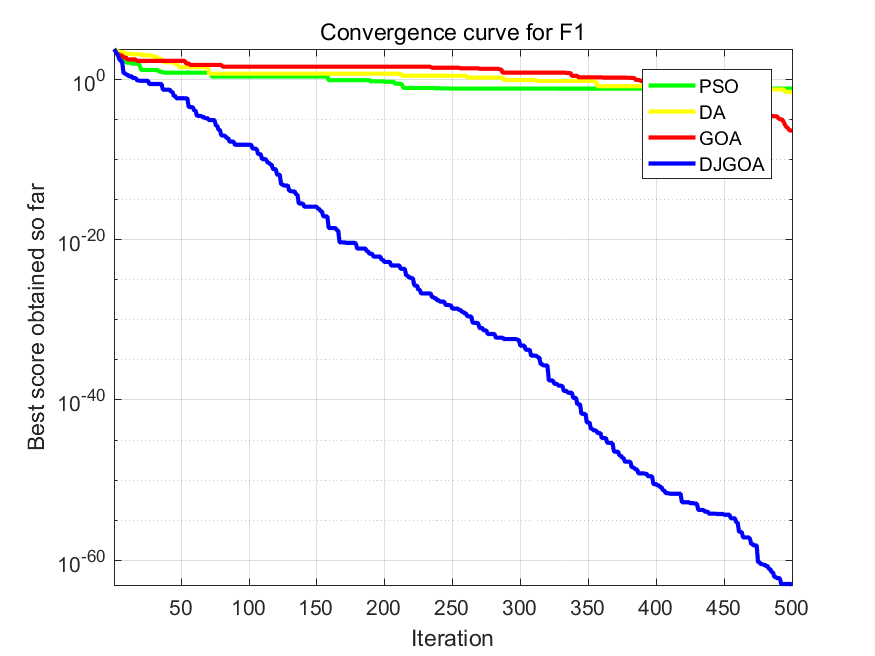
\includegraphics[width=.5\linewidth]{DJGOA_F1}\hfill
    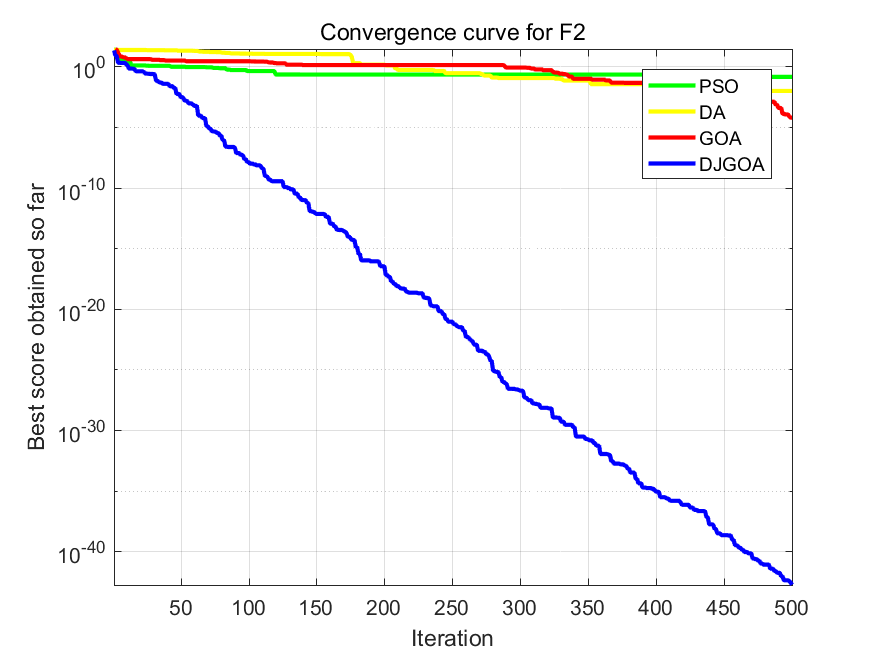
\includegraphics[width=.5\linewidth]{DJGOA_F2}\hfill\\[0.5cm]
    \centering
    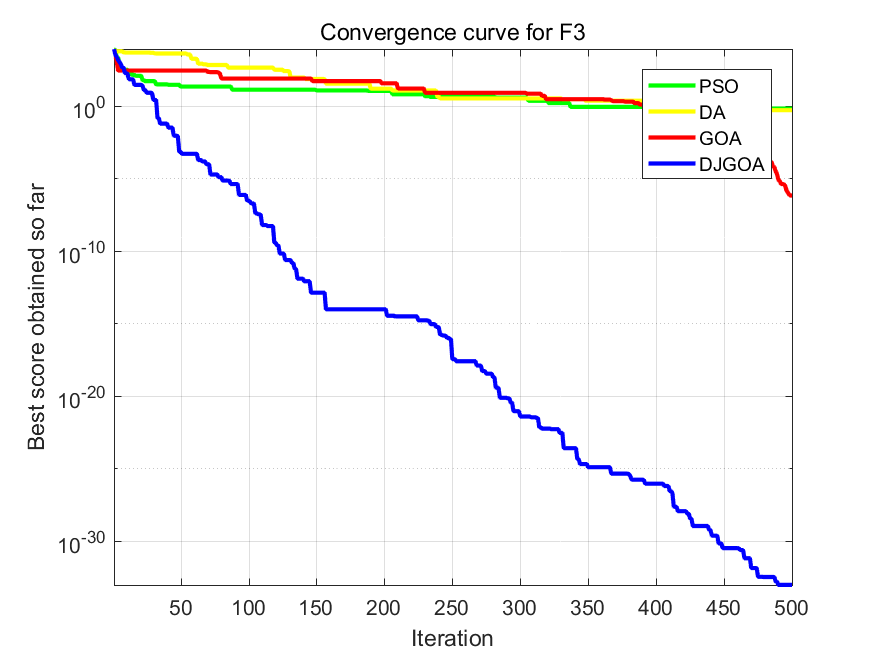
\includegraphics[width=.5\linewidth]{DJGOA_F3}\hfill
    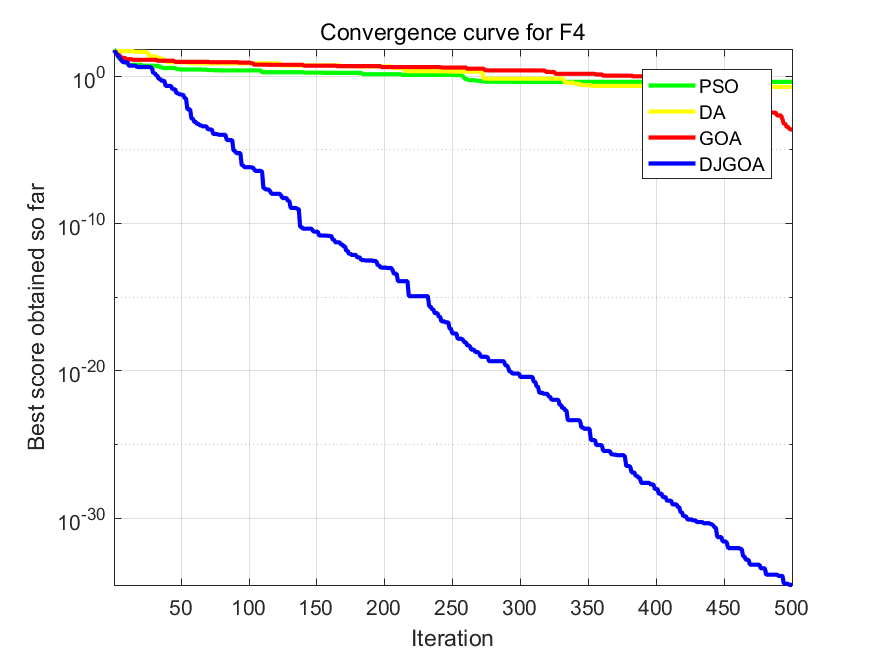
\includegraphics[width=.5\linewidth]{DJGOA_F4}\hfill\\[0.5cm]
    \centering
    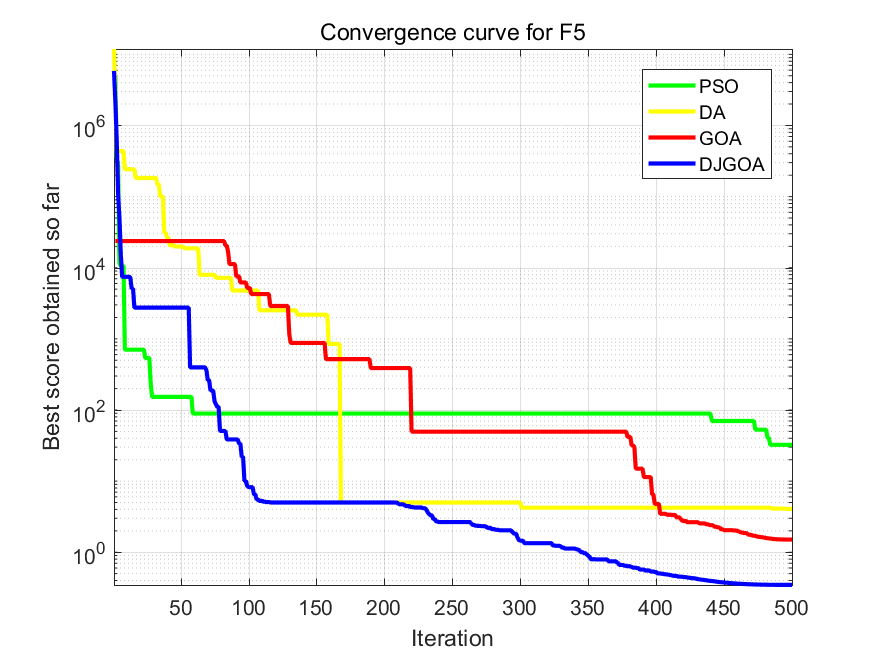
\includegraphics[width=.5\linewidth]{DJGOA_F5}\hfill
    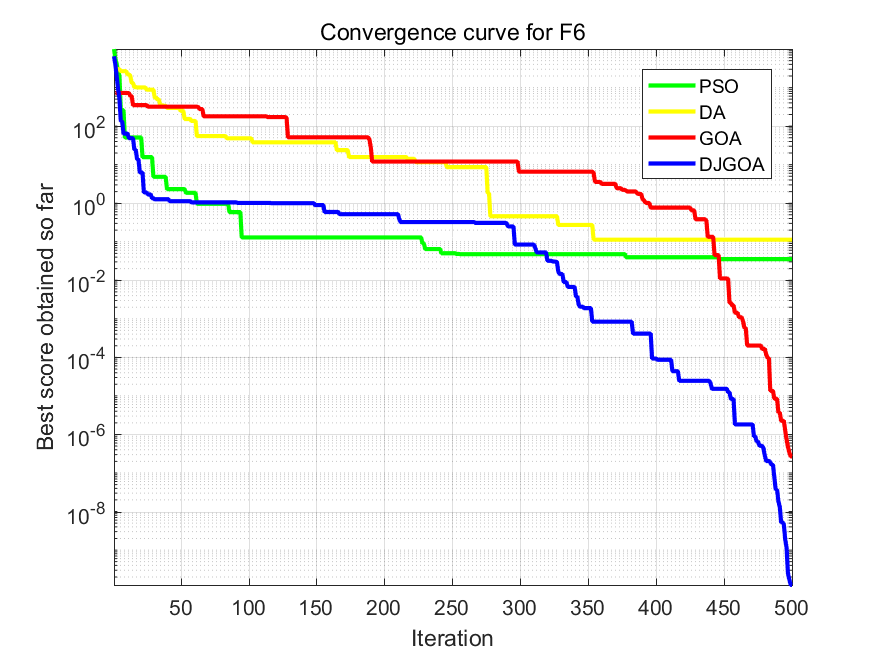
\includegraphics[width=.5\linewidth]{DJGOA_F6}\hfill\\[0.5cm]
    \caption{DJGOA、GOA、DA与PSO在13个测试函数上的收敛曲线}
    \label{fig:DJGOA_convergence_curve}
\end{figure}

\begin{figure}[!htbp]
    \ContinuedFloat
    \centering
    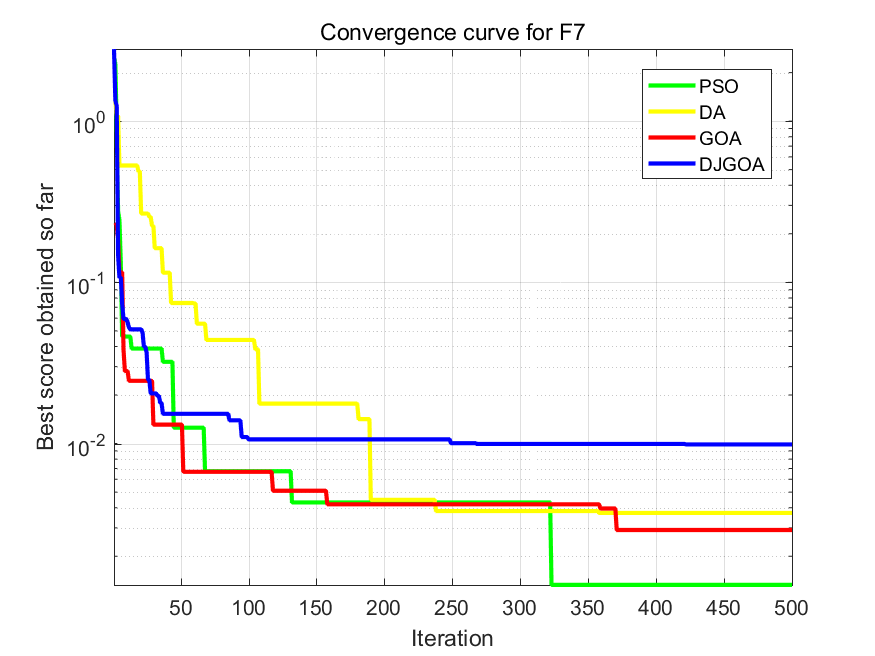
\includegraphics[width=.5\linewidth]{DJGOA_F7}\hfill
    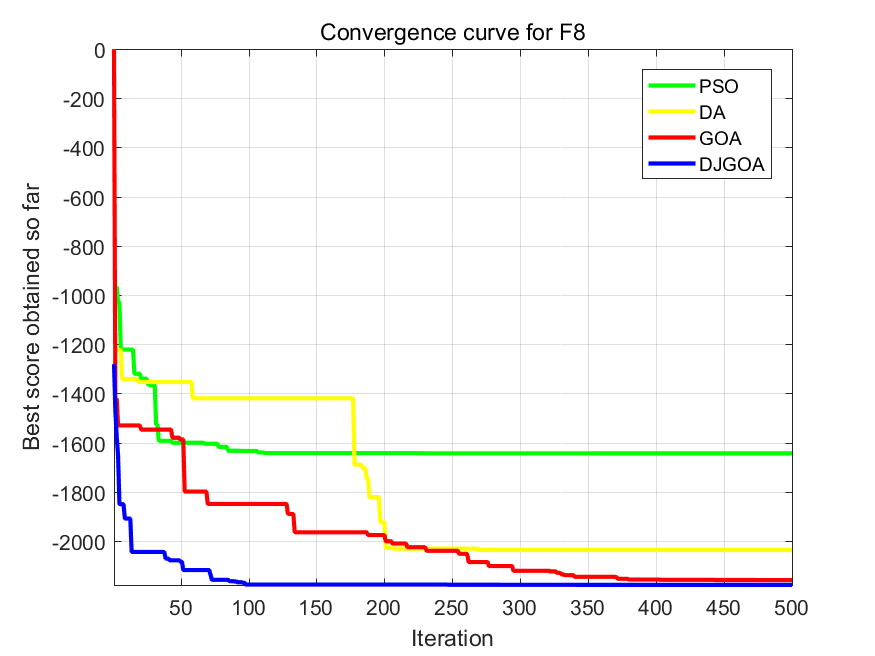
\includegraphics[width=.5\linewidth]{DJGOA_F8}\hfill\\[0.5cm]
    \centering
    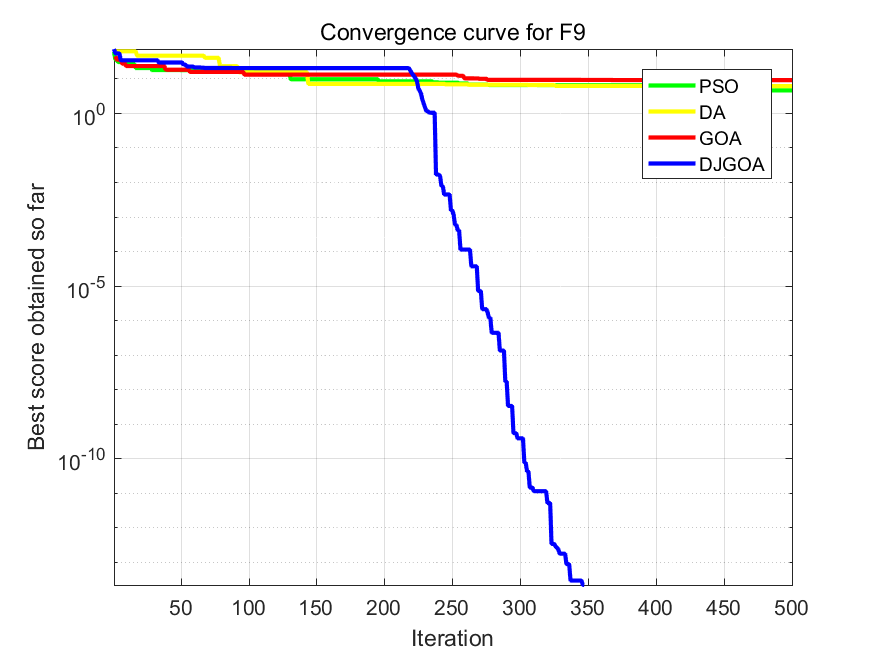
\includegraphics[width=.5\linewidth]{DJGOA_F9}\hfill
    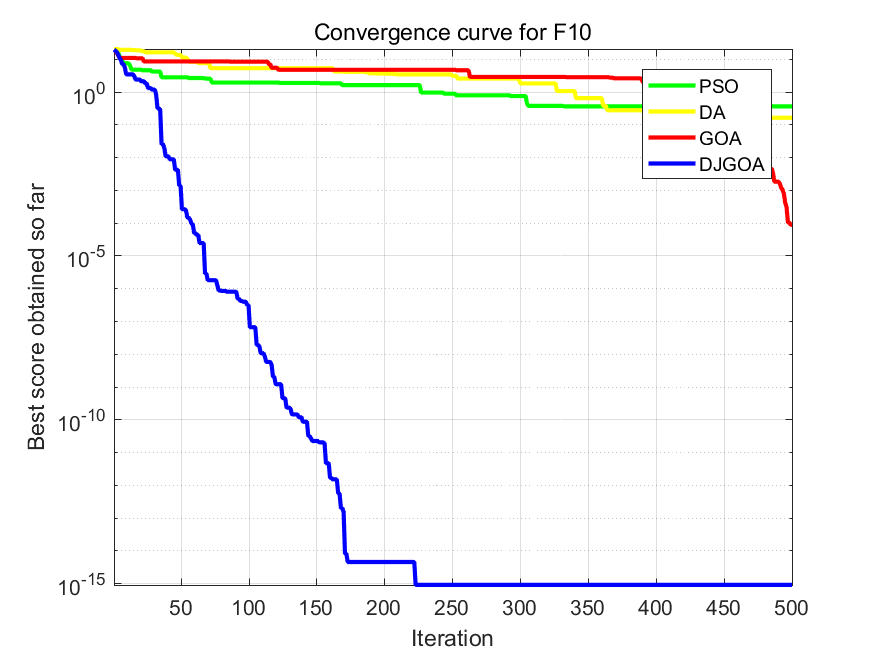
\includegraphics[width=.5\linewidth]{DJGOA_F10}\hfill\\[0.5cm]
    \centering
    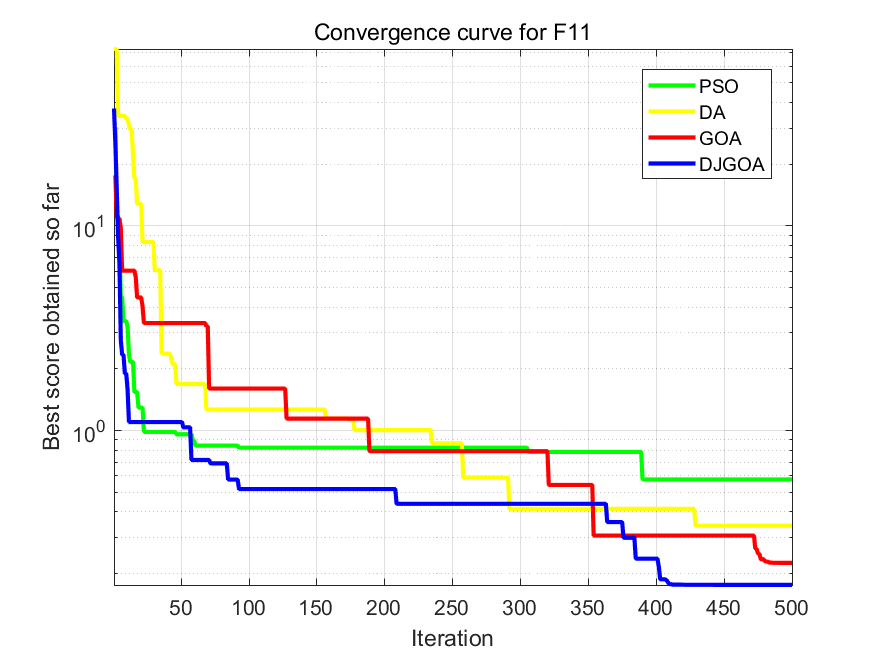
\includegraphics[width=.5\linewidth]{DJGOA_F11}\hfill
    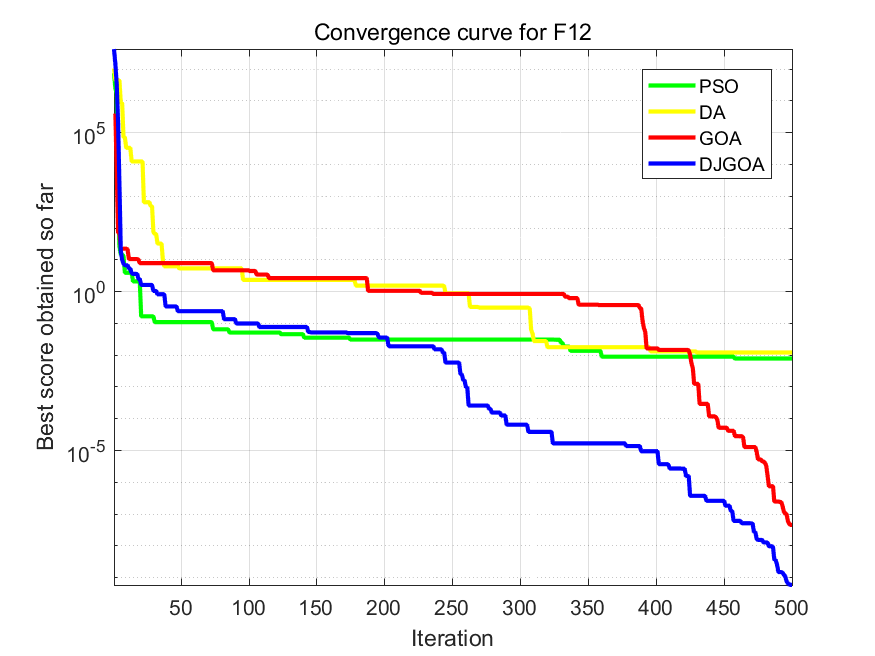
\includegraphics[width=.5\linewidth]{DJGOA_F12}\hfill\\[0.5cm]
    \centering
    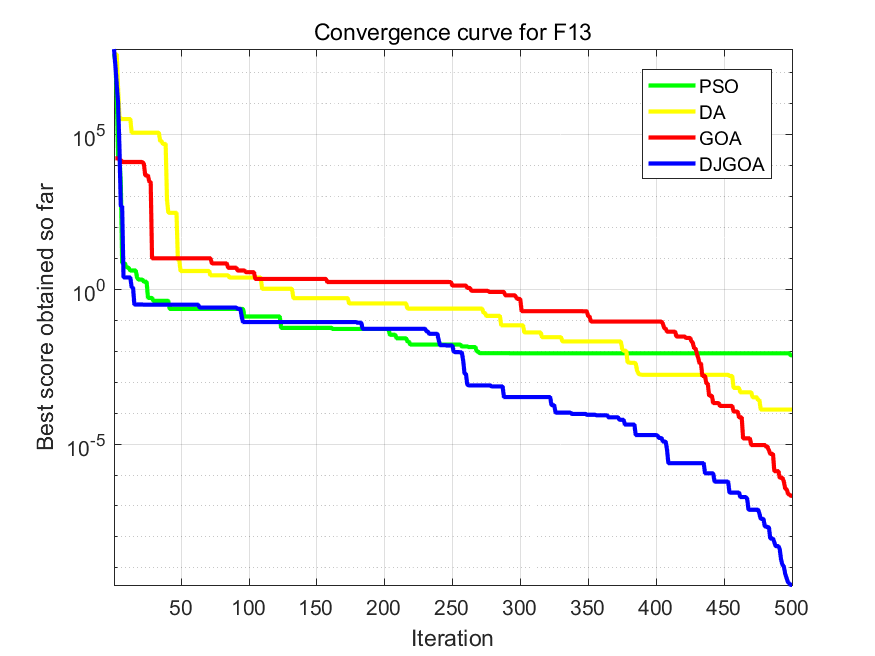
\includegraphics[width=.5\linewidth]{DJGOA_F13}\hfill\\[0.5cm]
    \caption{DJGOA、GOA、DA与PSO在13个测试函数上的收敛曲线(续)}
\end{figure}

\section{改进蝗虫优化算法(IGOA)}\label{sec:task_scheduling_IGOA}

如第\ref{sec:task_scheduling_DJGOA}小节所提到的,蝗虫优化算法具有简单的理论基础,易于实施,但同时它也还有一些阻碍算法找到更优解的缺点。线性减小的舒适区控制参数不能帮助原始的蝗虫优化算法充分利用每一次迭代。而且由于缺乏随机因素,原始的蝗虫优化算法几乎没有变化,这使得算法的搜索过程很容易陷入局部最优。为了解决这些不足,本小节在第\ref{sec:task_scheduling_DJGOA}小节所提出的DJGOA算法的基础上进一步引入了三个改进:非线性舒适区控制参数,基于$L\acute{e}vy $ flight的局部搜索机制和基于线性递减参数的随机跳出策略。本小节详细介绍了这三项改进工作的细节。

\subsection{非线性舒适区控制参数}
原始的蝗虫优化算法通过控制舒适区的半径使搜索单元一步步迭代,逐渐收敛到全局最优解附近。在搜索过程的探索阶段,舒适区控制参数应该足够大,以使搜索单元能够获得足够的搜索空间,以快速收敛到近似最优解的附近。在搜索过程中的开发阶段,舒适区控制参数应该较小,以使得搜索代理能够避免超速移动,并且能够在局部最优附近进行精确地搜索。线性递减的舒适区控制参数并不能做到使算法的搜索能力与迭代搜索期间经历的探索和开发这两个阶段协调一致。

为了使算法的搜索能力与两个搜索阶段相匹配并且增强算法在不同阶段的搜索能力,IGOA引入了sigmoid函数来作为舒适区的控制参数。sigmoid函数是常用的阈值函数和非线性调整因子。它被广泛应用于信息科学领域。sigmoid函数的表达式如公式\ref{equ:IGOA_sigmoid}所示。

\begin{eqnarray}\label{equ:IGOA_sigmoid}
	f(x)=\frac{1}{1+e^{-x}}
\end{eqnarray}

基于sigmoid函数变形的非线性舒适区控制参数表达式如公式\ref{equ:IGOA_sigmoid_comfort_parameter}所示。
% A nonlinear comfort zone parameter based on a variant of the sigmoid function is proposed as follows:
\begin{eqnarray}\label{equ:IGOA_sigmoid_comfort_parameter}
    m=\frac{-0.5}{1+e^{(-1.5(cx-5)+2\sin(cx))}}+w
\end{eqnarray}

在公式\ref{equ:IGOA_sigmoid_comfort_parameter}中,参数\emph{w}是调节参数,取值范围为[0,1]。参数\emph{cx}定义如公式\ref{equ:IGOA_cx}所示。
% where \emph{u} is the adjustment parameter and its value should be in the interval [0,1]. And \emph{cx} is defined as follows:
\begin{eqnarray}\label{equ:IGOA_cx}
	cx=\frac{v(iter+50)}{Maxiteration}
\end{eqnarray}

在公式\ref{equ:IGOA_cx}中,参数\emph{v}是精度调节参数,取值范围为[1,10]。
% where \emph{v} is the accuracy adjustment factor and its value should be in the interval [1,10].
\subsection{基于$L\acute{e}vy$飞行的局部搜索机制}

原始蝗虫优化算法中的所有参数都是确定性的,非常缺乏随机性。这会导致算法在搜索迭代演进的过程中缺乏创造性,每个搜索单元只能搜索相对确定的位置。将随机因子引入到确定性系统中是提高性能的常用的方法。
% All the parameters of GOA are deterministic. The lack of randomness might lead to the lack of creativity during the search iterations, and every search agent could only search the determinate position. Introducing random factor to a deterministic system is a commonly used method to improve its performance.

$L\acute{e}vy$飞行是由Paul $L\acute{e}vy$ \cite {mirjalili2016dragonfly}提出的一种随机搜索游走方法,是一种非常有效的提供随机因子的数学方法。由于$L\acute{e}vy$飞行实现起来非常复杂,所以研究人员通常使用一种模拟算法来代替$L\acute{e}vy$飞行,该方法的表达式如公式\ref{equ:IGOA_levy}所示。
% $L\acute{e}vy$ flight is a random search walk proposed by Paul $L\acute{e}vy$ \cite{mirjalili2016dragonfly}, and it is an efficient mathematical method to provide a random factor. Because $L\acute{e}vy$ flight is very complicated to implement, a simulating algorithm is used here as follows:
\begin{eqnarray}\label{equ:IGOA_levy}
	Levy(d)=0.01\times\frac{r_1\times\sigma}{|r_2|^{\frac{1}{\beta}}}
\end{eqnarray}

在公式\ref{equ:IGOA_levy}中,\emph{d}是要解决问题的维度,$r_1$和$r_2$是两个取值为[0,1]区间的随机数,$\beta$是一个常数,根据文献\cite{mirjalili2016dragonfly}的描述,通常取值为1.5。$\sigma$的计算方式如公式\ref{equ:IGOA_sigma}所示。
% where \emph{d} is the dimension of the problem, $r_1$,$r_2$ are two random numbers in [0,1] and $\beta$ is a constant number which is set to 1.5 according to Seyedali in \ cite{mirjalili2016dragonfly}. $\sigma$ is calculated as follows:
\begin{eqnarray}\label{equ:IGOA_sigma}
	\sigma=(\frac{\Gamma(1+\beta)\times \sin(\frac{\pi\beta}{2})}{\Gamma(\frac{1+\beta}{2})\time\beta\times2^(\frac{\beta-1}{2})})^\frac{1}{\beta}
\end{eqnarray}

在公式\ref{equ:IGOA_sigma}中,$\Gamma(x)=(x-1)!$。
% where $\Gamma(x)=(x-1)!$.

为了扩展搜索单元的搜索半径,增强算法的随机性以及局部最优值的搜索能力,本小节提出了一种基于$L\acute{e}vy$飞行的局部搜索机制。当一轮的位置更新过程结束的时候,可以以一定概率通过$L\acute{e}vy$飞行对每个搜索单元的位置进行调整。调整公式的定义如公式\ref{equ:IGOA_levy_flight}所示。在某种程度上,$L\acute{e}vy$飞行可以在搜索单元向着最优解位置搜索的过程中为其提供一定的“视觉”,使得搜索单元可以“看到”它们周围的一片较小的区域内的情况。

% $L\acute{e}vy$ flight could give vision to all the search agents when they are moving towards the optimal position. The search agents could see the small areas around them. To expand the search radius of the search agents and enhance the ability to find the optima, a local search mechanism based on $L\acute{e}vy$ flight is proposed. When a location updating process is finished, the position of every search agent should be adjusted through $L\acute{e}vy$ flight with a certain probability. The adjustment formula is defined as follows:
\begin{eqnarray}\label{equ:IGOA_levy_flight}
	X_i=X_i+10c\times s_{threshold}\times Levy(dim)\times X_i
\end{eqnarray}

在公式\ref{equ:IGOA_levy_flight}中,$s_{threshold}$是控制飞行方向和变化概率的阈值参数。$s_{threshold}$的计算方法如公式\ref{equ:IGOA_s_threshold}所示。
% where $s_{threshold}$ is the threshold parameter which control the direction and the probability of the variation. $s_{threshold}$ is calculated as follows:
\begin{eqnarray}\label{equ:IGOA_s_threshold}
	s_{threshold}=sign(x_{trans}-1)+sign(x_{trans}+1)
\end{eqnarray}

在公式\ref{equ:IGOA_s_threshold}中,$sign(x)$是sign符号函数,$x_{trans}$是取值在[-3,3]之间的随机数。
% where $sign(x)$ is the sign function and $x_{trans}$ is a random number in [-3,3].
\subsection{基于线性递减参数的随机跳出策略}

蝗虫优化算法的基础理论是初级的。该算法只关注了收敛到全局最优的过程,而忽略了跳出局部最优的机制。因此,蝗虫优化算法的搜索过程很容易陷入局部最优,使得搜索无法更进一步进行下去。

% The basic theory of GOA is elementary. The algorithm only focuses on the process of convergence to the global optimum and ignores the mechanism about jumping out of the local optimum. Hence the search process of GOA was easy to be trapped in local optimum, and the search could not go further. The advantage that GOA was simple to implement could not contribute to getting rid of the local optimum, which could be a disadvantage of GOA instead.

为了提高蝗虫优化算法的跳出局部最优的能力,本小节提出了基于线性递减参数的随机跳出策略。当搜索单元搜索到当前最优解的位置的时候,新的目标位置可以替换旧的目标位置。如果没有,则可以开始启动基于线性递减参数的随机跳出机制。该机制的方法如公式\ref{equ:IGOA_random_jumping}所示。
% To promote the capability to jump out of the local optimum, a random jumping strategy is introduced. When a search agent finds an optimal position, the new position can replace the old target position. When it does not, the random jumping equation is starting to work. It is described as follows:
\begin{eqnarray}\label{equ:IGOA_random_jumping}
	X_i^{new}=((0.5-rand)\times 2+1)X_i 
\end{eqnarray}

在公式\ref{equ:IGOA_random_jumping}中,$X_i$是第\emph{i}个搜索单元的位置,$X_i^{new}$是第\emph{i}个搜索单元进行随机跳出以后得到的新位置。如果$X_i^{new}$拥有更优的适应度值,那么它将会取代$X_i$。这样一次成功的跳出行为就发生了。
% where $X_i$ is the position of the \emph{i}-th search agent, and $X_i^{new}$ is the new position after random jumping. If $X_i^{new}$ has better fitness, it will replace $X_i$. Thus action of jumping out occurs successfully. 

原始蝗虫优化算法的演进公式仅仅将当前迭代获得的最佳位置作为搜索方向,但是忽略了一些其他可能有用信息。为了使新发生的成功跳出动作所能提供的信息的影响力持续下去,IGOA将搜索单元的位置迭代演进公式变成如公式\ref{equ:IGOA_evolution}所示。
% The evolution formula of the original GOA only takes the best position obtained by the current iteration as the search direction, and it ignores some other useful information. To continue the influence of the newly obtained information of the jumping action, the evolution formula of the location is transformed as follows:
\begin{eqnarray}\label{equ:IGOA_evolution}
	X_i^{iter+1}=m\times c\times S_i+(1-p)\widehat{T_d}+p\times X_i^{iter}
\end{eqnarray}

在公式\ref{equ:IGOA_evolution}中,\emph{p}是用于控制搜索单元位置影响的协调参数。\emph{p}在第一次迭代的时候初始化为0。 如果搜索单元没有进行跳出或者跳出局部最优失败,\emph{p}仍会被设置为0,以确保只有$S_i$和$T_d$才能影响下一次迭代演进。当搜索单元完成一次成功跳出时,\emph{p}被设置为在接下来的3次迭代中线性递减为0的变量,以使成功跳出的行为的影响持续到接下来的3次迭代演进过程中。经过一些试验,\emph{p}的递减间隔被设置为0.3478,并且本文并未对此取值进行详细的研究讨论。这样在本研究中,参数\emph{p}的计算方法如公式\ref{equ:IGOA_p}所示。
% where \emph{p} is the coefficient parameter to control the impact of the position of the search agent. \emph{p} is initialized as 0 at the first iteration. If the search agent does not jump or it fails to jump out of the local optimal location, \emph{p} is still set to 0 to make sure that the evolution can be affected only by $S_i$ and $T_d$. When the search agent jumps out successfully, \emph{p} is set to a variable linearly decreasing to 0 in three iterations to continue the influence of the behavior of jumping. After some trial, the decreasing step of \emph{p} is set to 0.3478 which is not discussed in this paper. Thus \emph{p} is calculated in this work as follows:
\begin{eqnarray}\label{equ:IGOA_p}
    p= \begin{cases}
        p-0.3478 & p>0 \\
        0&p \leq 0 \\
        3\times 0.3478&when \  jumping \  out \  successfully
        \end{cases} 
\end{eqnarray}

\subsection{改进蝗虫优化算法流程}

本小节中提出了一种改进的蝗虫优化算法。改进蝗虫优化算法的搜索过程分为初始化阶段,迭代演进阶段,适应度更新阶段和跳出阶段四个阶段。
% This paper proposed an Improved Grasshopper Algorithm (IGOA). The procedure of the IGOA is divided into four stages which were the initialization stage, the evolution stage, the fitness updating stage and the jumping stage. 

在初始化阶段,设置参数,并随机初始化所有搜索单元的初始位置。在这一阶段中,还计算了最优目标的位置和相应的最优适应度值。在迭代演进阶段,搜索循环开始进行。每个搜索单元都通过公式\ref{equ:IGOA_evolution}移动到新的位置。非线性舒适区参数\emph{m}根据公式\ref{equ:IGOA_sigmoid_comfort_parameter}进行设置。之后每个搜索单元根据公式\ref{equ:IGOA_levy_flight}以一定的概率进行$L\acute{e}vy$飞行调整,并生成新的搜索位置。在适应度值更新阶段,计算新位置的适应度值。如果新的适应度值优于当前的全局最优适应度值,则新的位置可以取代旧的全局最优目标的位置。如果新的适应度值没有比当前全局最优目标的适应度值更优,那么该搜索单元就会进入跳出阶段。在此阶段,搜索单元尝试根据公式\ref{equ:IGOA_random_jumping}跳出局部最优,并计算新的适应度值。如果新的适应度值优于当前搜索单元本身的适应度值,那么新的位置可以取代旧的搜索单元的位置,完成一次成功的跳出。此时参数\emph{p}也由根据公式\ref{equ:IGOA_p}进行更新。如果新的适应度值没有优于当前搜索单元本身的适应度值,那么搜索单元不会跳到新的位置上,会仍然停留在旧的位置上。到目前为止,循环求解过程中的一次迭代已经完成。在达到最大迭代次数之后,循环过程结束,此时的全局最优适应度值和全局最优目标位置就是最终的寻优求解的结果。改进蝗虫优化算法的伪代码算法图如算法\ref{alg:IGOA}所示。改进蝗虫优化算法的算法流程框图如图\ref{fig:procedure_IGOA}所示。
% In the initialization stage, the parameters are set, and the original positions of all the search agents are initialized randomly. The best target position and the corresponding fitness are also calculated in this part. The search loop starts to work in the evolution stage. Every search agent moves towards the target position by \emph{Equation 14}. The nonlinear comfort zone parameter \emph{m} is set by \emph{Equation 7}. After that, every search agent conducts $L\acute{e}vy$ flight in a particular probability by \emph{Equation 11} and a new position is generated. In the updating stage, the fitness of the new position is calculated. If the new fitness is better than the global fitness, the new position can replace the old global target. If the new fitness is not more optimal than the global target, it comes to the jumping stage. In this stage, the search agent tries to jump out of the local optimum by \emph{Equation 13} and a new fitness is calculated. If the new fitness is better than personal fitness, the new position can replace the old personal position. Parameter \emph{p} is updated by \emph{Equation 15} as well. So far, one iteration in the loop is finished. After the maximum number of iterations is reached, the loop ends, and the fitness and the target position are presented as the final result. The pseudo code of the IGOA is shown as \emph{Algorithm 1}. The figure framework of the procedure of IGOA is shown as \emph{Figure 1}.
\begin{algorithm}
    % \setstretch{1.35}
    \caption{改进蝗虫优化算法}
    \label{alg:IGOA}
    
    \begin{algorithmic}[1]
    
    \State 初始化参数
    \State 通过随机矩阵初始化蝗虫集群的初始位置
    \State 计算初始目标适应度值,记录目标位置
    
    \While {$(iter < MaxIteration$ 且 $target fitness > destination fitness)$}
    \State 根据公式\ref{equ:IGOA_sigmoid_comfort_parameter}设置非线性舒适区控制参数\emph{m}
    \State 根据公式\ref{equ:IGOA_evolution}更新$x_i$的位置
    \State $x_i$搜索单元根据公式\ref{equ:IGOA_levy_flight}进行$L\acute{e}vy$飞行
    \State 计算适应度值 
    \If{当前适应度值优于目标适应度值}
        \State 更新目标适应度值和目标最优解位置
    \Else
        \State $x_i$搜索单元根据公式\ref{equ:IGOA_random_jumping}进行跳出
        \State 计算适应度值
        \If{当前适应度值优于搜索单元自身适应度值}
            \State 更新搜索单元的位置
        \EndIf
        \State 根据公式\ref{equ:IGOA_p}设置参数\emph{p}的值
    \EndIf
    \EndWhile
    \State 返回得到的目标最优值和目标最优解的位置
    \end{algorithmic}
\end{algorithm}

\graphicspath{{Img/}}
\begin{figure}[htbp]
    \centering
    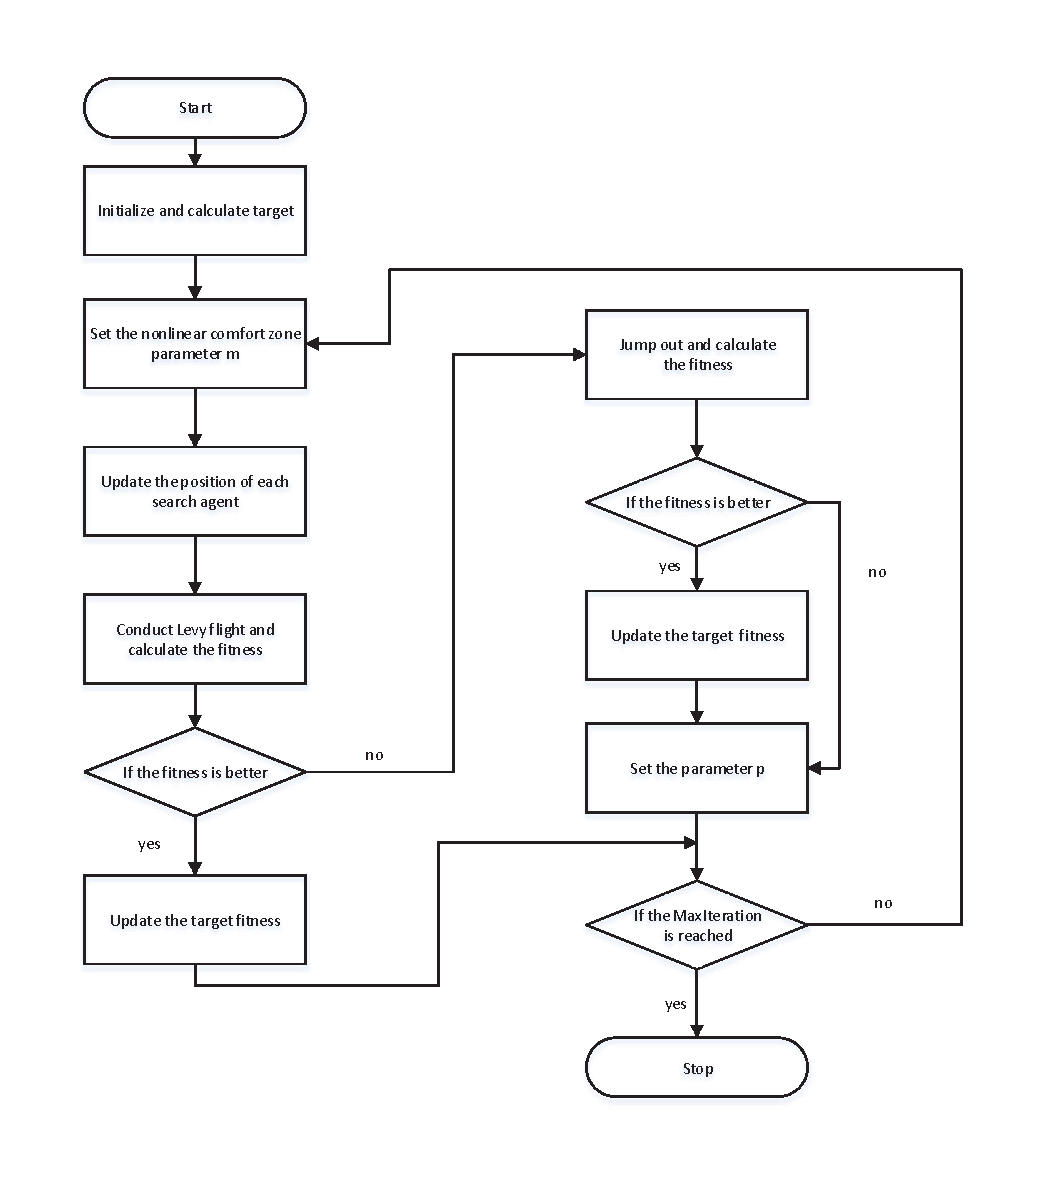
\includegraphics[width=1\linewidth]{procedure_of_IGOA.eps}\hfill\\[0.5cm]
  \caption{改进蝗虫优化算法的算法流程框图}
  \label{fig:procedure_IGOA}
\end{figure}
\subsection{实验结果}
\subsubsection{实验设置}

为了评估所提出的改进蝗虫优化算法(IGOA)的性能,本小节进行了一系列实验。在本小节的工作中,IGOA算法与6个元启发式算法的性能进行了比较,包括原始的蝗虫优化算法(GOA),基于反向学习的蝗虫优化算法(OBLGOA),最近几年新提出的三种元启发式算法,鲸鱼优化算法(WOA),蜻蜓优化算法(DA)和蚁狮优化算法(ALO),以及经典的启发式算法,粒子群优化算法(PSO)。在本小节的实验中,其他6种算法的参数设置如文献\cite{saremi2017grasshopper,ewees2018improved,mirjalili2016whale,mirjalili2016dragonfly,mirjalili2015ant,kennedy1995particle}所示。
% To evaluate the performance of the proposed IGOA, a series of experiments were conducted. In this work, IGOA was compared with 6 meta-heuristic algorithms including the original Grasshopper Optimization Algorithm (GOA), the opposition-based learning GOA (OBLGOA), three recently proposed algorithms, Whale Optimization Algorithm (WOA), Dragonfly Algorithm (DA) and Ant Lion Optimizer (ALO), and a classical heuristic algorithm, Particle Swarm Optimization (PSO). The parameters of the other 6 algorithms compared with IGOA were set as the papers \cite{saremi2017grasshopper,kennedy1995particle,mirjalili2016WOA,mirjalili2016dragonfly,ewees2018improved,mirjalili2015ant} described.
% 这里需要提一下IGOA的参数设置问题

本小节的实验使用了29个著名的benchmark测试函数来测试所提出的改进蝗虫优化算法的搜索性能。benchmark测试函数可以分为3种类型,用来评估算法的不同方面的性能。在表\ref{tab:unimodal_function}中列出的测试函数$F_1-F_7$是单峰测试函数,只有一个局部最优位置,也即是全局最优位置,可以用来评价算法的局部搜索能力。在表\ref{tab:multimodal_function}和表\ref{tab:fixedmodal_function}中列出的benchmark测试函数$F_8-F_{23}$是具有多个局部最优的多峰测试函数,可以用来评价算法的全局搜索能力\cite{saremi2017grasshopper}。在表\ref{tab:composite_function}中所列出的测试函数$F_{24}-F_{29}$是复合测试函数\cite{liang2005novel},复合测试函数在一种特定的框架内组合了一些基本的测试函数,得到更加复杂的测试函数。复合测试函数可以用来评价算法摆脱局部最优的能力。在表\ref{tab:unimodal_function}、表\ref{tab:multimodal_function}、表\ref{tab:fixedmodal_function}和表\ref{tab:composite_function}中,\emph{Dim}表示测试函数的维度,\emph{Range}是优化问题的搜索边界,$f_min$是测试函数的预期最优适应度值。在本小节的实验中,表\ref{tab:unimodal_function}和表\ref{tab:multimodal_function}中所列的测试函数$F_1-F_{13}$的维度均为30。
% In this part, 29 well-known benchmark functions were used to test the search ability of the proposed IGOA. The benchmarks are divided into 3 types which can evaluate the different capability of the algorithms. Benchmarks \emph{F1-F7} listed in \emph{Table 1} are unimodal functions with only one optimal location which can estimate the ability of exploitation. Benchmarks \emph{F8-F23} listed in \emph{Table 2} and \emph{Table 3} are multimodal functions with several local optimums which can evaluate the exploration capability \cite{saremi2017grasshopper}.  Benchmarks \emph{F24-F29} listed in \emph{Table 4} are composite functions \cite{liang2005novel} which combine some basic test functions under a framework and are more complicated. They can evaluate the performance of getting out of local optimum. In \emph{Table 1-4}, \emph{Dim} represents the dimension of the benchmark functions, \emph{Range} is the search boundary of the optimization problems, and $f_min$ is the optimal fitness of the functions.

使用Matlab代码在上述29个benchmark测试函数上完成了一系列相关实验。对于测试函数$F_1-F_{23}$,每个算法使用30个搜索单元搜索,每次实验进行500次迭代搜索。对于测试函数$F_{24}-F_{29}$,每次实验的搜索过程进行100次迭代。每次搜索实验对每个算法重复30次以降低意外情况的影响。通过计算一些30次实验的统计数据,例如平均值(avg),标准差(std),30次重复实验中得到的最优适应度值(best)和30次重复实验中得到的最差适应度值(worst),比较算法的性能。另外,还进行了威尔科克森秩和检验,计算了\emph{p-value}以证明实验结果的统计显著性。
% A series of experiments relating to the 29 benchmark functions described above were conducted with Matlab code. For \emph{F1-F23}, each algorithm was evolved for 500 iterations with 30 search agents to make a complete search process. For \emph{F24-F29}, a search process contained 100 iterations. Each search process would be repeated 30 times for every algorithm to eliminate contingency and some statistical data, such as average (avg), standard deviation (std), best fitness of 30 (best) and worst fitness of 30 (worst), was calculated to compare the performance of the algorithms. Besides, the Wilcoxon rank-sum test was conducted, and the \emph{p-value} was calculated to demonstrate the statistical significance of the results.

\begin{table}[!htbp]
    \centering
    \caption{多峰测试函数(续)}
    \label{tab:fixedmodal_function}
    \small
    \renewcommand\arraystretch{2.0} 
    \newcommand{\tabincell}[2]{\begin{tabular}{@{}#1@{}}#2\end{tabular}}
\begin{tabular}{l c c c}
    \hline
    % after \\: \hline or \cline{col1-col2} \cline{col3-col4} ...
    Function & Dim & Range & $f_{min}$ \\
    \hline
    $F_{14}(x)=(\frac{1}{500}+\sum_{j=1}^{25} \frac{1}{j+\sum_{i=1}^2 (x_i-a_{ij})^6})^{-1}$ & 2 & [-65,65]&0 \\
    \hline
    $F_{15}(x)=\sum_{i=1}^{11}[a_i-\frac{x_i(b_i^2+b_ix_2)}{b_i^2+b_ix_3+x_4}]^2$& 4 & [-5,5]&0.00030 \\
    \hline
    $F_{16}(x)=4x_1^2-2.1x_1^4+\frac{1}{3}x_1^6+x_1x_2-4x_2^2+4x_2^4$& 2 & [-5,5] & -1.0316\\
    \hline
    $F_{17}(x)=(x_2-\frac{5.1}{4\pi ^2}x_1^2+\frac{5}{\pi}x_1-6)^2+10(1-\frac{1}{8\pi})\cos x_1+10$& 2 & [-5,5] & 0.3979\\
    \hline
    \tabincell{c}{$F_{18}(x)= [1+(x_1+x_2+1)^2(19-14x_1+3x_1^2-14x_2+6x_1x_2+3x_2^2)]\times$ \\ $[30+2x_1-3x_2)^2\times(18-32x_1+12x_1^2+48x_2-36x_1x_2+27x_2^2)]$ }& 2 & [-2,2] & 3\\
    \hline
    $F_{19}(x)=-\sum_{i=1}^4c_iexp(-\sum_{j=1}^3a_{ij}(x_j-p_{ij})^2)$& 3 & [1,3] & -3.86\\
    \hline
    $F_{20}(x)=-\sum_{i=1}^4c_iexp(-\sum_{j=1}^6a_{ij}(x_j-p_{ij})^2)$& 6 & [0,1] & -3.32\\
    \hline
    $F_{21}(x)=-\sum_{i=1}^5[(X-a_i)(X-a_i)^T+c_i]^{-1}$& 4 & [0,10] & -10.1532\\
    \hline
    $F_{22}(x)=-\sum_{i=1}^7[(X-a_i)(X-a_i)^T+c_i]^{-1}$& 4 & [0,10] & -10.4028\\
    \hline
    $F_{23}(x)=-\sum_{i=1}^10[(X-a_i)(X-a_i)^T+c_i]^{-1}$& 4 & [0,10] & -10.5363\\
    \hline
\end{tabular}
\end{table}

\begin{table}[!htbp]
    \centering
    \caption{复合测试函数}
    \label{tab:composite_function}
    \scriptsize
    % \small

\newcommand{\tabincell}[2]{\begin{tabular}{@{}#1@{}}#2\end{tabular}}
    \renewcommand\arraystretch{1.5} 
\begin{tabular}{l c c c}
    \hline
    % after \\: \hline or \cline{col1-col2} \cline{col3-col4} ...
    Function & Dim & Range & $f_{min}$ \\
    \hline
    \tabincell{l}{$F_{24}(CF1)$ \\$f_1,f_2,f_3,...f_{10}=Sphere Function,[\sigma_1,\sigma_2,\sigma_3,...\sigma_{10}=[1,1,1,...1]$\\$[\lambda_1,\lambda_2,\lambda_3,...\lambda_{10}]=[5/100,5/100,5/100,...5/100]$}& 30 & [-5,5]&0 \\
    \hline
    \tabincell{l}{$F_{25}(CF2)$ \\$f_1,f_2,f_3,...f_{10}=Griewank's Function,[\sigma_1,\sigma_2,\sigma_3,...\sigma_{10}=[1,1,1,...1]$\\$[\lambda_1,\lambda_2,\lambda_3,...\lambda_{10}]=[5/100,5/100,5/100,...5/100]$}& 30 & [-5,5]&0 \\
    \hline
    \tabincell{l}{$F_{26}(CF3)$ \\$f_1,f_2,f_3,...f_{10}=Griewank's Function,[\sigma_1,\sigma_2,\sigma_3,...\sigma_{10}=[1,1,1,...1]$\\$[\lambda_1,\lambda_2,\lambda_3,...\lambda_{10}]=[1,1,1,...1]$}& 30 & [-5,5]&0 \\
    \hline
    \tabincell{l}{$F_{27}(CF4)$ \\$f_1,f_2=Ackley's Function,f_3,f_4=Rastrigin's Function,$\\$f_5,f_6=Weierstrass Function,f_7,f_8=Griewank's Function,$\\$f_9,f_{10}=Sphere Function,[\sigma_1,\sigma_2,\sigma_3,...\sigma_{10}=[1,1,1,...1]$\\$[\lambda_1,\lambda_2,\lambda_3,...\lambda_{10}]=[5/32,5/32,5/32,...5/32]$}& 30 & [-5,5]&0 \\
    \hline
    \tabincell{l}{$F_{28}(CF5)$ \\$f_1,f_2=Rastrigin's Function,f_3,f_4=Weierstrass Function,$\\$f_5,f_6=Griewank's Function,f_7,f_8=Ackley's Function,$\\$f_9,f_{10}=Sphere Function,[\sigma_1,\sigma_2,\sigma_3,...\sigma_{10}=[1,1,1,...1]$\\$[\lambda_1,\lambda_2,\lambda_3,...\lambda_{10}]=[1/5,1/5,5/0.5,5/0.5,5/100,5/100,5/32,5/32,5/100,5/100]$}& 30 & [-5,5]&0 \\
    \hline
    \tabincell{l}{$F_{29}(CF6)$ \\$f_1,f_2=Rastrigin's Function,f_3,f_4=Weierstrass Function,$\\$f_5,f_6=Griewank's Function,f_7,f_8=Ackley's Function,$\\$f_9,f_{10}=Sphere Function$\\$[\sigma_1,\sigma_2,\sigma_3,...\sigma_{10}=[0.1,0.2,0.3,0.4,0.5,0.6,0.7,0.8,0.9,1]$\\$[\lambda_1,\lambda_2,\lambda_3,...\lambda_{10}]=[0.1*1/5,0.2*1/5,0.3*5/0.5,0.4*5/0.5,0.5*5/100,$\\$0.6*5/100,0.7*5/32,0.8*5/32,0.9*5/100,1*5/100]$}& 30 & [-5,5]&0 \\
    \hline
  \end{tabular}

\end{table}
\subsubsection{实验结果}
函数$F_1-F_7$是单峰函数,只有一个局部最优解,也即是全局最优解,可以用来测试算法的局部搜索能力。如果搜索算法具有超强的局部开发能力,它可以进行更精确的搜索,并找到更接近全局最优的解。函数$F_1-F_7$的实验结果显示在表\ref{tab:results_unimodal_IGOA}中。
% \emph{F1-F7} are unimodal functions with only one global optimum, which can test the exploitation capability of the algorithms. If an algorithm has a superior ability of exploitation, it can search more accurately and find a solution closer to the global optimum. 


\begin{table}[!htbp]
    \centering
    \caption{$F_1-F_7$单峰测试函数实验结果}\label{tab:results_unimodal_IGOA}
    \scriptsize
    % \small
    \renewcommand\arraystretch{1.3} 
    \begin{tabular}{*{9}{c}}
    % \toprule
    \hline
    function& type&IGOA&GOA&WOA&DA&ALO&PSO&OBLGOA\\
    \hline
\multirow{4}*{F1}& avg& 3.3538E-15& 0.8386& \textbf{1.0082E-71}& 0.0012& 17.1234&6.6310E-6&2.77E-05\\
    & std&1.9129E-15&0.8473&\textbf{5.3671E-71}&0.0008&17.8648&2.1612E-05&1.57E-05    \\
    & best&8.0120E-16&0.0683&\textbf{5.0175E-87}&0.00010&2.4120&1.5608E-07&7.75E-06    \\
    & worst& 9.1885E-15&4.4591&\textbf{2.9415E-70}&0.0030&78.3488&0.0001&6.68E-05    \\
    \hline
\multirow{4}*{F2}& avg& 2.4358E-08& 10.2444&\textbf{ 1.5782E-51}& 47.0419& 4.9289&0.0953&0.0136\\
    & std&1.0173E-08&22.2516&\textbf{4.8668E-51}&43.4815&3.7734&3.0196E-01&0.0377    \\
    & best&9.0029E-09&0.0290&\textbf{2.5368E-57}&3.8197&1.4484&0.0003&0.0011    \\
    & worst&5.7194E-08&79.1046&\textbf{2.1838E-50}&120.4026&21.3472&1.6419&0.1505    \\
    \hline
\multirow{4}*{F3}& avg&0.0121& 1789.3452&43942.9825&4632.0793&1154.2060&227.7776 &\textbf{0.0061}\\
    & std&0.0211&	1030.4488&1.6119E+04&2008.3302&1332.5907&81.0377&\textbf{0.0021}    \\
    & best&\textbf{8.6626E-12}&450.4535&17269.6957&1883.2010&249.1874&127.3043&0.0020    \\
    & worst&0.0983&4603.9086&85296.2126&10156.9819&5729.0798&425.9704&\textbf{0.0103}    \\
    \hline
\multirow{4}*{F4}& avg&0.0257&9.7756&56.3543&16.9378&31.4847&3.2311&\textbf{0.0165}\\
    & std&0.0182&3.5013&25.3903&4.3129&8.2314&1.1774&\textbf{0.0081}    \\
    & best&\textbf{9.7116E-7}&3.0335&3.2199&6.5808&17.7108&1.4918&0.0010    \\
    & worst&0.0694&19.5647&89.1869&57.2014&48.8229&5.5785&\textbf{0.0297}    \\
    \hline
\multirow{4}*{F5}& avg&\textbf{26.4488}&965.6578&28.1591&348.5174&1615.4578&61.9257&28.3790\\
    & std&\textbf{0.3046}&1572.3600&0.4797&553.5976&2814.6516&64.9991&0.3087    \\
    & best&25.8503&25.6988&27.2726&28.4537&143.9488&\textbf{1.7275}&27.6749    \\
    & worst&\textbf{27.0365}&7522.9967&28.7708&2223.6927&14636.9499&268.0065&28.7678    \\
    \hline
\multirow{4}*{F6}& avg&\textbf{1.4451E-6}& 0.8997&0.3866&0.0023&20.5677&2.2973E-05&1.2542\\
    & std&\textbf{4.8437E-7}&2.0343&0.2498&0.0055&29.2793&5.0099E-05&0.4237    \\
    & best&\textbf{5.2803E-7}&0.0203&0.0856&0.0001&3.0268&1.5390E-07&0.6616    \\
    & worst& \textbf{2.5210E-6}&11.0963&1.0626&0.0306&148.1366&0.0002&2.1687    \\
    \hline
\multirow{4}*{F7}& avg& \textbf{0.0010}&0.0234&0.0032&0.2504&0.1588&0.0274&0.0014\\
    & std&\textbf{0.0014}&0.0106&0.0032&0.0768&0.0934&0.0113&0.0007    \\
    & best&\textbf{1.0746E-5}&0.0090&5.1138E-5&0.1003&0.0467&0.0115&0.0006    \\
    & worst&0.0072&0.0602&0.0118&0.4105&0.3750&0.0538&\textbf{0.0033}    \\
    \hline
    % \bottomrule
    \end{tabular}
    \end{table}

从表\ref{tab:results_unimodal_IGOA}中可以看出,IGOA可以在函数$F_5-F_7$中获得最佳的平均值结果,并且在函数$F_1-F_4$中,IGOA的表现也仅比WOA差。关于标准差和最差值方面,IGOA也可以比函数$F_3-F_7$中的其他算法表现更好,这表明所提出的算法可以降低获得更差解的可能性并且提高算法的稳定性。与GOA和OBLGOA相比,所提出的IGOA可以显著提高原蝗虫优化算法的局部开发搜索能力。
% The results on \emph{F1-F7} are shown in \emph{Table 5}. It could be seen that IGOA could get the best average results in \emph{F5-F7}, and in \emph{F1-F4} IGOA behaved only worse than WOA. As for std and worst value, IGOA could also perform better than the other algorithms in \emph{F3-F7}, which indicates that the proposed algorithm can reduce the probability of getting terrible solutions and promote the stability of the algorithm. Compared with GOA and OBLGOA, the proposed IGOA can significantly improve the exploitation capability of the original algorithm.  

函数$F_8-F_{23}$是具有多个局部最优解的多峰测试函数,可以测试算法的全局探索能力。如果搜索算法在搜索的过程中不能完成得很好,那么在处理多峰测试函数时,搜索很可能会陷入局部最优,即使拥有更好的局部开发能力也不能帮助算法取得更好的结果。错误的努力方向可能会导致错误的结果。函数$F_8-F_{23}$的实验结果如表\ref{tab:results_multimodal_IGOA}和表\ref{tab:results_fixedmodal_IGOA}所示。
% \emph{F8-F23} are multimodal functions with several local optimums, which can test the exploration capability of the algorithms. If an algorithm cannot do well in exploration, the search will most likely fall into local optimum when dealing with the multimodal functions and even the best ability of exploitation cannot help. A wrong direction can probably lead to a wrong result. 


\begin{table}[!htbp]
    \centering
    \caption{$F_8-F_{13}$多峰测试函数实验结果}\label{tab:results_multimodal_IGOA}
    \scriptsize
    % \small
    \renewcommand\arraystretch{1.3} 
    \begin{tabular}{*{9}{c}}
        % \toprule
    \hline
    function& type&IGOA&GOA&WOA&DA&ALO&PSO&OBLGOA\\
    \hline
    \multirow{4}*{F8}&avg & -7594.1662 & -7728.4324 & \textbf{-9969.6875} & -6189.11 & -7320.0609 & -6688.3058&-7901.9216\\
        & std & 767.0277 & \textbf{593.4825} & 1919.0327 & 1833.8338 & 886.1388 & 684.8647&591.8701    \\
        & best & -9009.3177 & -8903.0523 & -12564.8051 & \textbf{-12568.5831} & -9628.8472 & -7869.7845&-9598.7278    \\
        & worst& -5993.9317 & -6468.5651 & -5709.2023 & -5417.6748 & -6101.1009 & -5224.2865&\textbf{-6823.4703}    \\
        \hline
    \multirow{4}*{F9}& avg& \textbf{0.0000} & 9.4853 & 0.4119 & 8.8883 & 7.4670 & 4.5109&1.7919\\
        & std& \textbf{0.0000} & 5.4604 & 1.6505 & 4.5100 & 4.1855 & 2.8231 &2.1937    \\
        & best& \textbf{0.0000} & 1.9899 & 0.0000 & 0.9950 & 0.9959 & 0.9950 &4.42E-09    \\
        & worst& \textbf{0.0000} & 27.8586 & 8.1471 & 16.9143 & 16.9159 & 10.9445&6.9648    \\
        \hline
    \multirow{4}*{F10}& avg& 1.30e-08 & 3.0892 & \textbf{4.56e-15} & 5.0040 & 9.9207 & 1.3594&0.0010\\
        & std& 3.13e-09 & 0.8305 & \textbf{2.18e-15} & 3.1845 & 3.9783 & 0.8583&0.0002    \\
        & best& 8.58e-09 & 1.5021 & \textbf{8.88e-16} & 1.1582 & 3.3950 & 0.0002&0.0005    \\
        & worst& 1.97e-08 & 4.5855 & \textbf{7.99e-15} & 12.3302 & 16.3216 & 2.8857&0.0015    \\
        \hline
    \multirow{4}*{F11}& avg& \textbf{5.50e-15} & 0.6966 & 0.0069 & 0.0610 & 1.1803 & 0.0258&0.0002\\
        & std& \textbf{5.71e-15} & 0.1924 & 0.0379 & 0.0268 & 0.1822 & 0.0354&8.83E-05    \\
        & best& \textbf{6.66e-16} & 0.3226 & 0.0000 & 0.0068 & 1.041 & 9.58e-07&7.36E-05    \\
        & worst& \textbf{2.52e-14} & 1.0411 & 0.2076 & 0.1151 & 1.9360 & 0.1590&0.0004    \\
        \hline
    \multirow{4}*{F12}& avg& \textbf{8.93e-08} & 5.6658 & 0.0242 & 14.9630 & 25.6688 & 0.5808&0.0347\\
        & std& \textbf{3.28e-08} & 2.3767 & 0.0162 & 7.2414 & 14.1457 & 0.8898&0.0211    \\
        & best& \textbf{4.62e-08} & 1.8994 & 0.004 & 6.9778 & 6.3337 & 1.89e-07&0.0051    \\
        & worst& \textbf{1.85e-07} & 9.7664 & 0.0832 & 35.5319 & 55.4036 & 3.4350&0.1028    \\
        \hline
    \multirow{4}*{F13}& avg& \textbf{0.0138} & 8.7624 & 0.6039 & 24.9054 & 261.6986 & 0.2117&0.4087\\
        & std& \textbf{0.0298} & 9.0372 & 0.2536 & 15.4205 & 1186.8265 & 0.5112&0.2177    \\
        & best& \textbf{4.85e-07} & 0.3005 & 0.1459 & 0.3854 & 1.3788 & 9.86e-07&0.1211    \\
        & worst& \textbf{0.0989} & 35.2838 & 1.2995 & 56.9980 & 6534.7729 & 2.0239&1.1019    \\
        \hline
        % \bottomrule
    \end{tabular}
\end{table}
\begin{table}[!htbp]
    \centering
    \caption{$F_{14}-F_{23}$多峰测试函数实验结果}\label{tab:results_fixedmodal_IGOA}
    \scriptsize
    % \small
    \renewcommand\arraystretch{1.3} 
    \begin{tabular}{*{9}{c}}
        % \toprule
    \hline
    function& type&IGOA&GOA&WOA&DA&ALO&PSO&OBLGOA\\
    \hline
    \multirow{4}*{F14}&avg & 3.5566& \textbf{0.9980} & 2.7622 & 2.2142 & 1.7242 & 4.5076&3.0103\\
        & std & 2.9933 & \textbf{6.4341e-16} & 3.3587 & 2.1646 & 1.2701 & 3.0100&1.5672    \\
        & best & \textbf{0.9980} & 0.9980 & 0.9980 & 0.9980 & 0.9980 & 0.9980&0.9980    \\
        & worst & 10.7632    & \textbf{0.9980} & 10.7632 & 10.7632 & 5.9288 & 12.6705&5.9288    \\
        \hline
    \multirow{4}*{F15}& avg& \textbf{0.0003}& 0.0071 & 0.0007 & 0.0032 & 0.0029 & 0.0038&0.0063\\
        & std& \textbf{3.24E-05}    & 0.0089 & 0.0005 & 0.0062 & 0.0059 & 0.0076&0.0087    \\
        & best& \textbf{0.0003} & 0.0007 & 0.0003 & 0.0006 & 0.0003 & 0.0003&0.0003    \\
        & worst& \textbf{0.0004}    & 0.0204 & 0.0022 & 0.0206 & 0.0204 & 0.0204&0.0210    \\
        \hline
    \multirow{4}*{F16}& avg& \textbf{-1.0316} & -1.0316 & -1.03162 & -1.0316 & -1.0316 & -1.0316&-1.0316\\
        & std& \textbf{4.44E-16}    & 8.1630e-13 & 1.6137e-09 & 1.0917e-13 & 5.1620e-07 & 6.5195e-16&4.63E-06    \\
        & best & \textbf{-1.0316} & -1.0316 & -1.0316 & -1.0316 & -1.0316 & -1.0316&-1.0316    \\
        & worst& \textbf{-1.0316} & -1.0316 & -1.0316 & -1.0316 & -1.0316 & -1.0316&-1.0316    \\
        \hline
    \multirow{4}*{F17}& avg& \textbf{0.3979} & 0.3979 & 0.3979 & 0.3979 & 0.3979 & 0.3979&0.3979\\
        & std& \textbf{0}    & 7.3750e-13 & 8.4140e-06 & 2.1005e-14 & 1.0879e-06 & 0.0000 &1.82E-06    \\
        & best& \textbf{0.3979} & 0.3979 & 0.3979 & 0.3979 & 0.3979 & 0.3979&0.3979    \\
        & worst& \textbf{0.3979} & 0.3979 & 0.3979 & 0.3979 & 0.3979 & 0.3979&0.3979 \\
        \hline
    \multirow{4}*{F18}&avg & \textbf{3.0000} & 8.4000 & 3.0000 & 3.0000 & 3.0000 & 3.0000&3.0000\\
        & std& 4.11E-08    & 20.5503 & 7.0794e-05 & 6.2232e-13 & 7.7233e-06 & \textbf{6.0036e-16}&3.07E-10    \\
        & best& \textbf{3.0000} & 3.0000 & 3.0000 & 3.0000 & 3.0000 & 3.0000&3.0000\\
        & worst& \textbf{3.0000} & 84.0000 & 3.0003 & 3.0000 & 3.0000 & 3.0000&3.0000 \\
        \hline
    \multirow{4}*{F19}& avg& \textbf{-3.8628}& -3.7288 & -3.8582 & -3.8628 & -3.8628 & -3.8628&-3.8628\\
        & std& 1.67E-10    & 0.3062 & 0.0054 & 2.4040e-13 & 2.2464e-05 & \textbf{2.6402e-15}&2.95E-05    \\
        & best& \textbf{-3.8628} & -3.8628 & -3.8628 & -3.8628 & -3.8628 & -3.8628&-3.8628  \\
        & worst& \textbf{-3.8628}    & -2.7847 & -3.8408 & -3.8628 & -3.8627 & -3.8628&-3.8627 \\
        \hline
    \multirow{4}*{F20}& avg& -3.2863& \textbf{-3.2943} & -3.2364 & -3.2621 & -3.2819 & -3.2783&-3.2295\\
        & std& 0.0554    & \textbf{0.0511} & 0.1007 & 0.0610 & 0.0577 & 0.0584&0.1062    \\
        & best& \textbf{-3.3220} & -3.3220 & -3.3213 & -3.3220 & -3.3220 & -3.3220&-3.3220    \\
        & worst& \textbf{-3.2031} & -3.2031 & -3.0184 & -3.1981 & -3.1974 & -3.1996&-3.0334    \\
        \hline
        \hline
    \end{tabular}
\end{table}
\begin{table}[!htbp]
    \ContinuedFloat% continue splited float
    \centering
    \caption{续表:$F_{14}-F_{23}$多峰测试函数实验结果}\label{tab:results_fixedmodal_IGOA}
    \small
    \renewcommand\arraystretch{1.3} 
    \begin{tabular}{*{9}{c}}
    \multirow{4}*{F21}& avg& \textbf{-8.2870}& -6.0675 & -8.5287 & -5.8753 & -6.6400 & -5.9796&-7.2158\\
        & std& \textbf{2.4947}    & 3.6827 & 2.7585 & 3.0237 & 3.2604 & 3.3646&3.3058    \\
        & best& \textbf{-10.1532} & -10.1532 & -10.1498 & -10.1532 & -10.1532 & -10.1532&-10.1532    \\
        & worst& \textbf{-5.0552} & -2.6305 & -2.6292 & -2.6305 & -2.6305 & -2.6305&-2.6303    \\
        \hline
    \multirow{4}*{F22}& avg& \textbf{-9.3413}& -7.1190 & -7.2448 & -7.1785 & -5.1249 & -5.5091&-8.0724\\
        & std& \textbf{2.1597}    & 3.6556 & 3.0850 & 3.3668 & 2.5737 & 3.1769&3.1972    \\
        & best& \textbf{-10.4029} & -10.4029 & -10.4020 & -10.4029 & -10.4029 & -10.4029&-10.4029    \\
        & worst& \textbf{-5.0877}    & -1.8376 & -1.8352 & -1.8376 & -2.7517 & -1.8376&-2.7658    \\
        \hline
    \multirow{4}*{F23}& avg& -7.9281& -4.9279 & -6.5554 & -6.6569 & -5.4597 & -4.7287&\textbf{-8.0791}\\
        & std& \textbf{2.8536}    & 3.2796 & 3.3755 & 3.7558 & 3.0183 & 3.2997&3.5845    \\
        & best& \textbf{-10.5364} & -10.5364 & -10.5348 & -10.5364 & -10.5364 & -10.5364&-10.5364    \\
        & worst& \textbf{-3.8354} & -2.4217 & -1.6721 & -2.4217 & -2.4217 & -2.4273&-2.4217    \\
        \hline
        % \bottomrule
    \end{tabular}
\end{table}
从表\ref{tab:results_multimodal_IGOA}和表\ref{tab:results_fixedmodal_IGOA}中可以看出,所提出的IGOA可以在16个测试函数中的11个中获得最优的平均适应度值,并且在测试函数$F_{10}$、$F_{20}$和$F_{23}$中IGOA可以获得次优的结果。 关于标准差的实验结果表明,IGOA的稳定性可能不如在平均适应度值方面所表现的那么好,但在大多数测试中IGOA仍然是所有7种算法中最好的。关于最佳适应度值和最差适应度值的实验结果可以表明,所提出的IGOA具有在几乎所有测试函数的实验中寻找到最优解的可靠能力,并且IGOA找到最差解的概率也是最小的。与原始GOA以及OBLGOA相比,所提出的IGOA可以极大提高算法的搜索性能。
% The results on \emph{F8-F23} are presented in \emph{Table 6} and \emph{Table 7}. It can be found that the proposed IGOA can get the best average fitness in 11 of 16 benchmark tests and in \emph{F10}, \emph{F20} and \emph{23} IGOA can get the second best result. The results about standard deviation show that the stability of IGOA might not be as excellent as it shows in average fitness, but it still is the best of all the 7 algorithms in most of the tests. The results on best fitness and worst fitness can show that the proposed IGOA has the most reliable ability to find the best solution in almost all the benchmark tests and get the minimum probability to find the worst solution. In comparison with the original GOA and OBLGOA, the proposed IGOA can naturally enhance the performance of exploration of the algorithm a lot.


函数$F_{24}-F_{29}$是复合测试函数,复合测试函数在一种特定的框架内组合了一些基本的测试函数,来构建新的、复杂的、可控的测试函数。复合测试函数比多峰测试函数更加复杂,也更具挑战性,在评估算法的搜索能力时更有说服力。复合测试函数的实验结果如表\ref{tab:results_composite_IGOA}所示:
% \emph{F24-F29} are the composite test functions, which combine some basic benchmark functions under a particular framework to construct new controllable test functions. The composite benchmark functions are more complicated and more challenging than multimodal test functions, and they are more convincing when evaluating the search capability of an algorithm. 


\begin{table}[!htbp]
    \centering
    \caption{$F_{24}-F_{29}$复合测试函数实验结果}\label{tab:results_composite_IGOA}
    \scriptsize
    % \small
    \renewcommand\arraystretch{1.3} 
\begin{tabular}{*{9}{c}}
    % \toprule
    \hline
    function& type&IGOA&GOA&WOA&DA&ALO&PSO&OBLGOA\\
    \hline
\multirow{4}*{F24}& avg& \textbf{94.0428} & 135.9242 & 341.2250 & 1098.8600 & 189.5840 & 326.5899&189.6304\\
    & std& 130.6690 & 127.0964 & 164.2449 & \textbf{99.4449} & 117.6155 & 149.6609&83.2598    \\
    & best& \textbf{3.3965} & 29.6057 & 163.2687 & 796.3368 & 72.0563 & 118.9426&92.1210    \\
    & worst& 504.8393 & 514.7878 & 844.9761 & 1261.1685 & 554.4573 & 717.0723&\textbf{411.3461}    \\
    \hline
\multirow{4}*{F25}& avg& 324.3197 & \textbf{284.6066} & 521.9304 & 1211.2487 & 413.5431 & 393.6293&472.0768\\
    & std& 151.6351 & 163.1829 & 130.9867 & \textbf{94.2232} & 156.9269 & 126.4408&143.6411    \\
    & best& \textbf{21.2736} & 28.9418 & 244.2571 & 1006.3367 & 72.6341 & 161.9665&66.0628    \\
    & worst& \textbf{497.3555} & 510.3606 & 673.6729 & 1354.7747 & 662.1609 & 610.8645&606.4133    \\
    \hline
\multirow{4}*{F26}& avg& \textbf{525.7384} & 624.5092 & 1052.0733 & 1547.6195 & 884.9306 & 608.4939&875.4033\\
    & std& 128.5247 & 176.1401 & 155.6153 & 155.8894 & 157.8576 & \textbf{103.4249}&151.2467    \\
    & best& 317.4166 & \textbf{200.8044} & 849.0492 & 1064.4776 & 644.6867 & 326.5611&627.7263    \\
    & worst & 900.011 & 1196.9114 & 1351.5909 & 1710.9641 & 1222.5593 & \textbf{828.4274}&1217.9587    \\
    \hline
\multirow{4}*{F27}& avg& 894.6861 & 945.6744 & 902.6182 & 1421.5043 & 929.5948 & \textbf{757.5836}&895.7587\\
    & std& 29.1104 & 101.1013 & \textbf{15.0373} & 46.9584 & 128.2259 & 114.6504&34.7088    \\
    & best& 740.5569 & 638.304 & 896.3862 & 1319.5644 & 650.1341 & \textbf{538.8135}&719.3590    \\
    & worst& \textbf{900.0053} & 1030.5605 & 982.1588 & 1519.1409 & 1066.455 & 1012.7758 &953.3374    \\
    \hline
\multirow{4}*{F28}& avg & 304.9727 & \textbf{142.0615} & 456.9052 & 1354.378 & 194.2336 & 303.9595&497.1264\\
    & std& 367.9136 & \textbf{102.2128} & 255.4945 & 127.0279 & 182.4486 & 143.7137&351.6947    \\
    & best& \textbf{46.3796} & 54.2782 & 179.8317 & 992.2916 & 87.2393 & 113.7433&110.5681    \\
    & worst& 900.0040 & \textbf{435.4893} & 900.0000 & 1505.6248 & 1025.2583 & 675.3012&900.0049    \\
    \hline
\multirow{4}*{F29}& avg& 900.0003 & 907.4664 & \textbf{900.0000} & 1371.4241 & 925.7089 & 931.1013&900.0004 \\
    & std& 0.0001 & 5.1380 & \textbf{0.0000} & 56.4060 & 7.5901 & 19.0467&0.0002\\
    & best& \textbf{900.0000} & 901.0860 & 900.0000 & 1254.6648 & 913.0986 & 910.3009&900.0001 \\
    & worst& 900.0006 & 920.7888 & \textbf{900.0000} & 1000.7252 & 1000.7252 & 1000.7252&900.0009\\
    \hline
    % \bottomrule
\end{tabular}
\end{table}

根据表\ref{tab:results_composite_IGOA}中列出的$F_{24}-F_{29}$复合测试函数实验结果,可以看出,与其他6种算法相比,所提出的IGOA非常有竞争力。在测试函数$F_{24}$和$F_{26}$中,IGOA可以获得最优的平均适应度值,在测试函数$F_{25}$、$F_{27}$和$F_{29}$中IGOA可以获得次优的平均适应度值。在标准差方面,IGOA表现得不是最好的,也不是最差的。IGOA在最优值和最差值方面,分别在4个函数和3个函数中表现最佳。尽管IGOA在标准差方面表现得一般,但它在寻找更优解、避免更差解以及控制风险方面可以胜过其他算法。与原始GOA和OBLGOA相比,IGOA的性能能够提升很多。根据复合函数的测试的结果,可以证明所提出的IGOA算法具有处理这种复杂而具有挑战性的问题的能力。

\subsubsection{威尔科克森秩和检验}

基于30次独立实验的平均值和标准差没有比较每次实验之间的差异。所得到的实验结果仍有可能包含某些意外情况。为了消除这种偶然性并证明实验结果的显著性,本小节引入了威尔科克森秩和检验。威尔科克森秩和检验是零假设的非参数检验,它用于确定两个独立的数据集是否来自相同的分布群体。本小节计算了关于IGOA与每个其他算法之间在测试函数$F_1-F_{29}$上的统计数据的\emph{p-values}。当\emph{p-value}小于0.05时,可以认为两个样本之间的差异是显著的。IGOA的威尔科克森秩和检验结果如表\ref{tab:results_wilcoxon_rank_sum_test_IGOA}所示。
% The comparison based on average value and standard deviation for 30 independent operations did not compare the difference between each operation. It was still possible that the results of the experiment contained certain contingency. To dispel this contingency and demonstrate the significance of the results of the experiment, the Wilcoxon rank-sum test was introduced in this work. Wilcoxon rank-sum test is a nonparametric test of the null hypothesis, and it is used to determine whether two independent datasets were from the same distributed population. In this work, \emph{p-values} about the statistical data between IGOA and each of the other algorithms on \emph{F1-F29} were calculated. When \emph{p-value} is less than 0.05, it can be considered that the difference between the two samples is significant.

\begin{table}[ht]
    \centering
    \caption{测试函数$F_1-F_{29}$的威尔科克森秩和检验结果}\label{tab:results_wilcoxon_rank_sum_test_IGOA}
    \renewcommand\arraystretch{1.3} 

	% \tiny

    \begin{tabular}{*{7}{c}}
    % \toprule
    \hline
    function&GOA&WOA&DA&ALO&PSO&OBLGOA\\
    \hline
 
    {F1}& 3.02E-11&3.02E-11&3.02E-11&3.02E-11&9.53E-07&2.03E-07\\\hline
    {F2}& 3.02E-11&3.02E-11&3.02E-11&3.02E-11&7.12E-09&2.37E-10\\\hline
    {F3}& 3.02E-11&3.02E-11&3.02E-11&3.02E-11&3.02E-11&5.57E-10\\\hline
    {F4}& 3.02E-11&3.02E-11&3.02E-11&3.02E-11&3.02E-11&1.21E-10\\\hline
    {F5}& 1.86E-09&1.60E-07&3.02E-11&3.02E-11&0.5201&5.07E-10\\\hline
    {F6}& 3.02E-11&3.02E-11&3.02E-11&0.0099&3.02E-11&3.02E-11\\\hline
    {F7}& 3.16E-10&0.7618&3.02E-11&3.02E-11&8.15E-11&0.0594\\\hline
    {F8}& 0.0030&3.82E-09&0.7958&2.59E-06&0.0133&0.0002\\\hline
    {F9}& 3.02E-11&1.24E-09&3.02E-11&3.02E-11&2.86E-11&4.98E-11\\\hline
    {F10}& 3.02E-11&3.02E-11&3.02E-11&3.02E-11&1.43E-08&3.83E-05\\\hline
    {F11}& 3.02E-11&4.56E-11&3.02E-11&3.02E-11&1.34E-05&3.02E-11\\\hline
    {F12}& 3.02E-11&3.02E-11&3.02E-11&3.02E-11&0.0002&3.02E-11\\\hline
    {F13}& 3.02E-11&3.02E-11&3.02E-11&3.02E-11&0.9117&3.02E-11\\\hline
    {F14}& 1.67E-05&0.1578&0.0265&0.0082&0.7842&0.6951\\\hline
    {F15}& 1.33E-10&1.07E-09&2.87E-10&2.87E-10&0.3328&2.15E-10\\\hline
    {F16}& 0.0064&6.72E-10&3.02E-11&1.81E-05&4.08E-12&3.02E-11\\\hline
    {F17}& 3.20E-06&3.01E-11&3.01E-11&6.78E-06&4.56E-12&3.01E-11\\\hline
    {F18}& 1.73E-07&3.02E-11&3.02E-11&0.01911&1.55E-11&5.09E-08\\\hline
    {F19}& 0.5997&0.002266&2.13E-05&3.33E-11&5.14E-12&0.0003\\\hline
    {F20}& 0.5395&0.0003&0.00250&0.7958&0.0003&0.0001\\\hline
    \end{tabular}
\end{table}
\begin{table}[ht]
    \ContinuedFloat% continue splited float
    \centering
    \caption{续表:测试函数$F_1-F_{29}$的威尔科克森秩和检验结果}\label{tab:results_wilcoxon_rank_sum_test_IGOA}
    % \scriptsize
    % \small
    \renewcommand\arraystretch{1.3} 
    \begin{tabular}{*{7}{c}}
    {F21}& 0.0002&1.25E-05&6.74E-06&0.0850&0.2822&5.46E-06\\\hline
    {F22}& 0.0005&5.27E-05&3.83E-06&0.5493&0.0627&0.0013\\\hline
    {F23}& 6.05E-07&3.83E-06&1.73E-06&0.1858&0.0009&5.27E-05\\\hline
    {F24}& 0.0016&6.01E-08&0.0001&3.02E-11&3.81E-07&0.0001\\\hline
    {F25}& 0.7618&1.09E-05&0.0138&3.02E-11&0.1907&1.02E-05\\\hline
    {F26}& 0.0046&5.49E-11&5.57E-10&3.02E-11&0.0038&4.20E-10\\\hline
    {F27}& 7.74E-06&7.34E-09&0.0064&3.02E-11&3.08E-08&2.68E-06\\\hline
    {F28}& 0.3711&0.0042&0.0083&3.02E-11&0.0073&0.0001\\\hline
    {F29}& 3.02E-11&2.14E-11&3.02E-11&3.02E-11&3.02E-11&0.0024\\\hline
    
    % \bottomrule
\end{tabular}
\end{table}

从表\ref{tab:results_wilcoxon_rank_sum_test_IGOA}中可以看出,在大多数的测试中,IGOA与另外的比较算法之间的\emph {p-values}小于0.05,实验所得到的结论是显著的。在某些测试函数中,某些\emph{p-values}超过了0.05,但这些函数中不同的算法会获得相同的最优解,例如测试函数$F_{14}$、$F_{19}$、$F_{20}$、$F_{21}$、$F_{22}$和$F_{23}$。通过分析复合函数的实验结果,在测试函数$F_{25}$和$F_{28}$中,\emph{p-values}在IGOA和GOA之间超过0.05,但是其中GOA能够找到最佳适应度值而IGOA却没有。综合考虑,仍然可以证明所提出的IGOA可以显著提高算法的性能。
% From \emph{Table 9} it can be seen that the \emph{p-values} between IGOA and another compared algorithm in most of the benchmark tests are less than 0.05. Some \emph{p-values} are more than 0.05 in some of the test functions which have a higher probability of achieving the same optimal solution by different algorithms, such as \emph{F14,F19,F20,F21,F22,} and \emph{F23}. By analyzing the results of the composite functions, \emph{p-values} are more than 0.05 between IGOA and GOA in \emph{F25} and \emph{F28} where GOA gets the best fitness and IGOA does not. Considering comprehensively, it can still be demonstrated that the proposed IGOA can significantly promote the performance of GOA.
\subsubsection{算法测试收敛速度}

本小节讨论了算法的收敛速度。IGOA和所有其他6种算法在部分测试函数上搜索的收敛曲线图如图\ref{fig:IGOA_convergence_curve}所示。
% \pagestyle{empty}
\graphicspath{{Img/}}
\begin{figure}[ht]
    \centering

    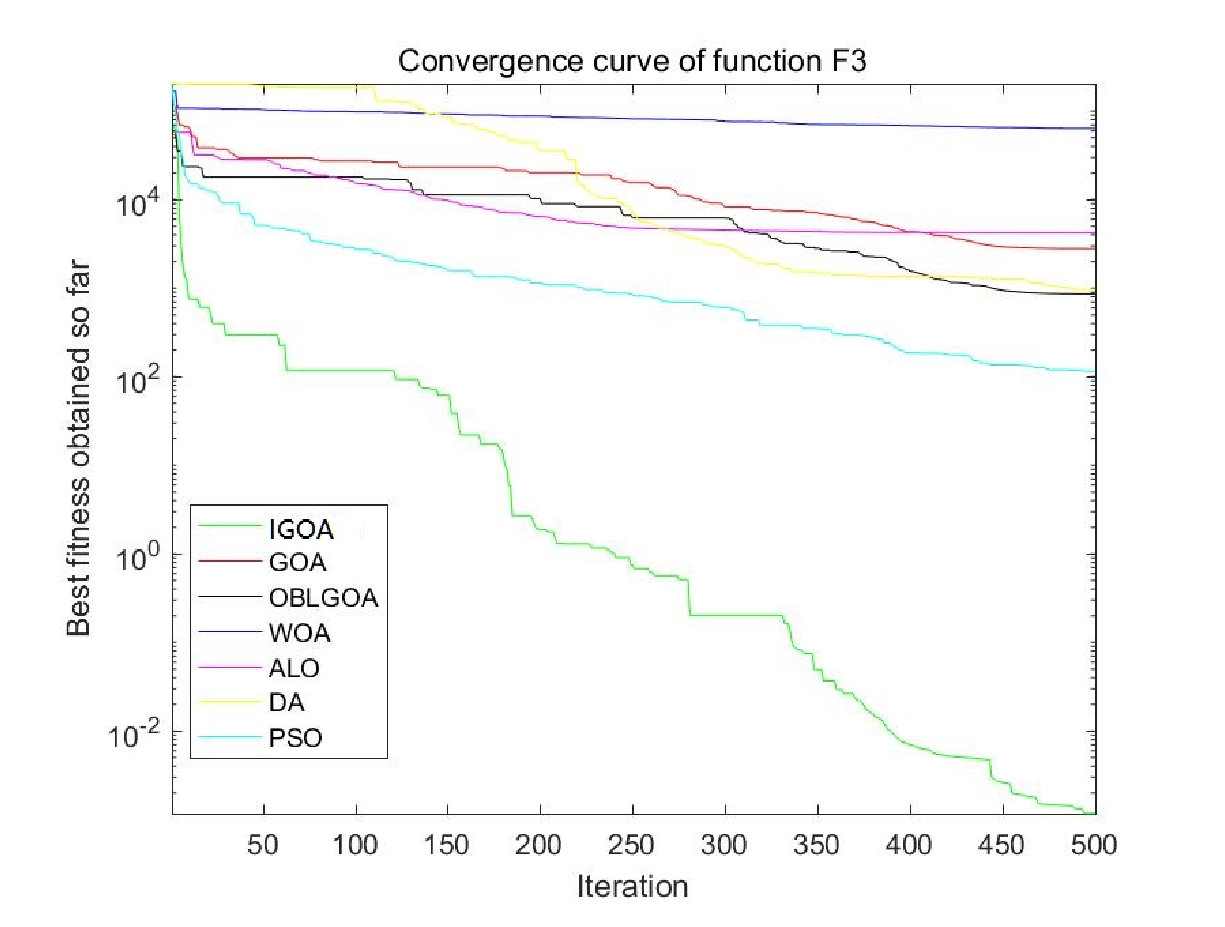
\includegraphics[width=.5\linewidth]{function_F3.eps}\hfill
    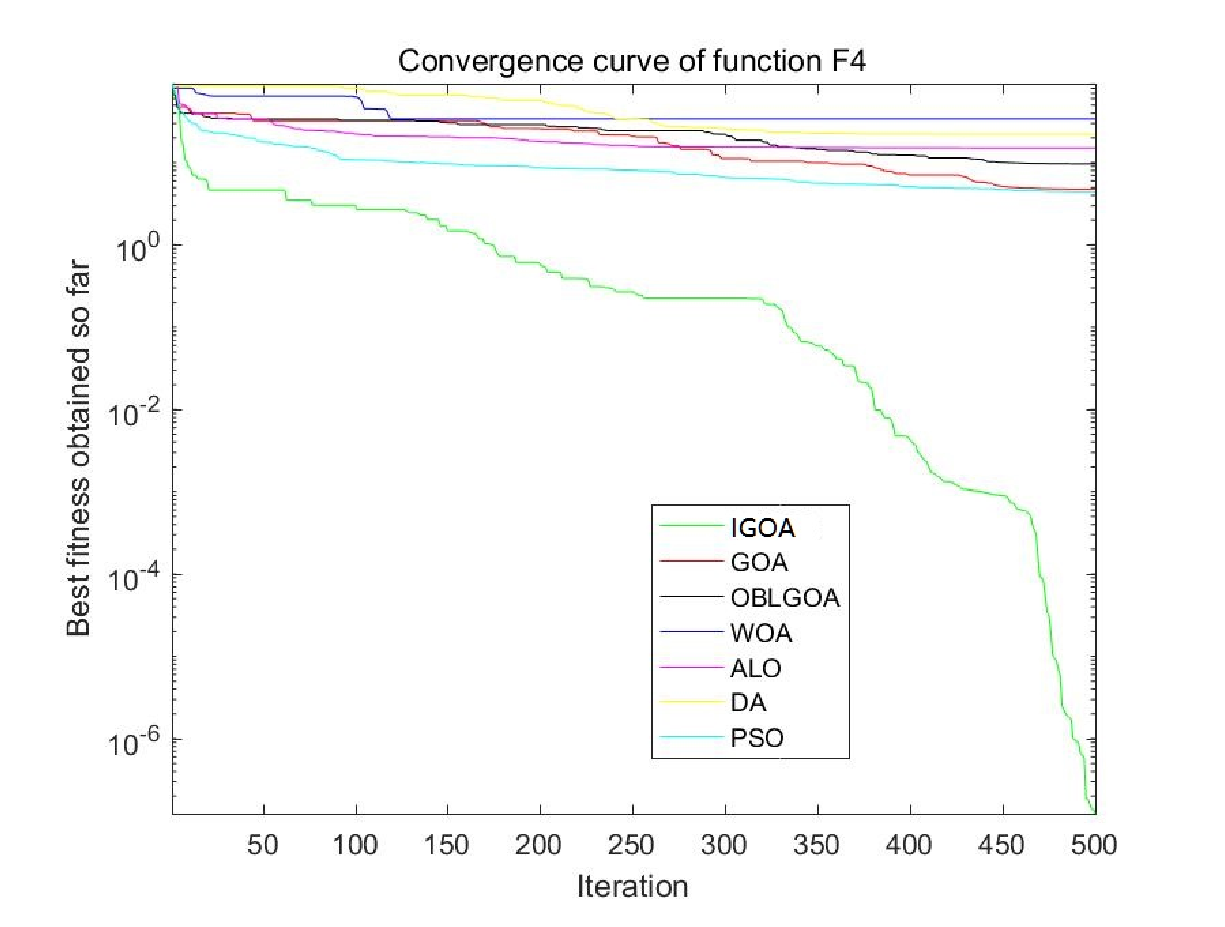
\includegraphics[width=.5\linewidth]{function_F4.eps}\hfill\\[0.5cm]

    \centering
    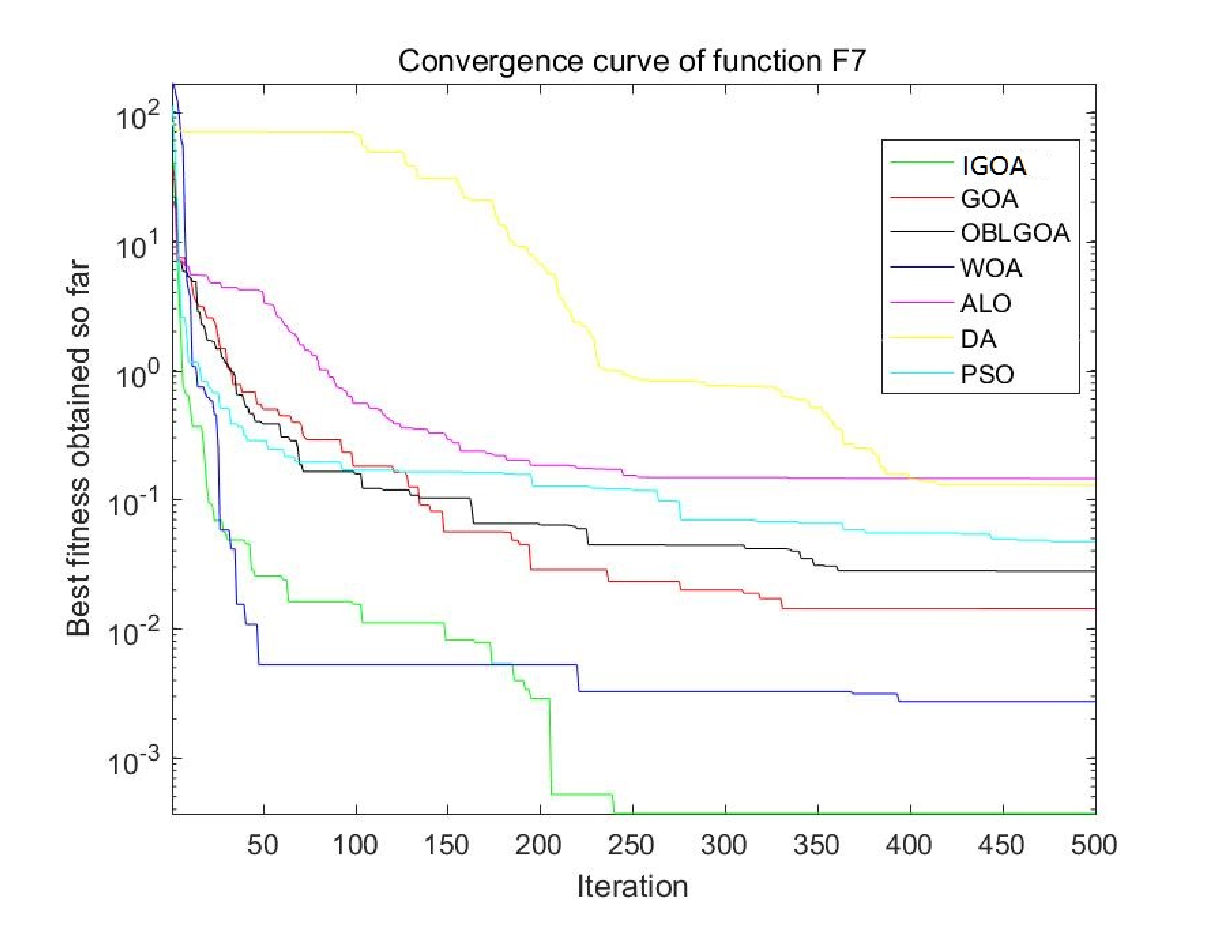
\includegraphics[width=.5\linewidth]{function_F7.eps}\hfill
    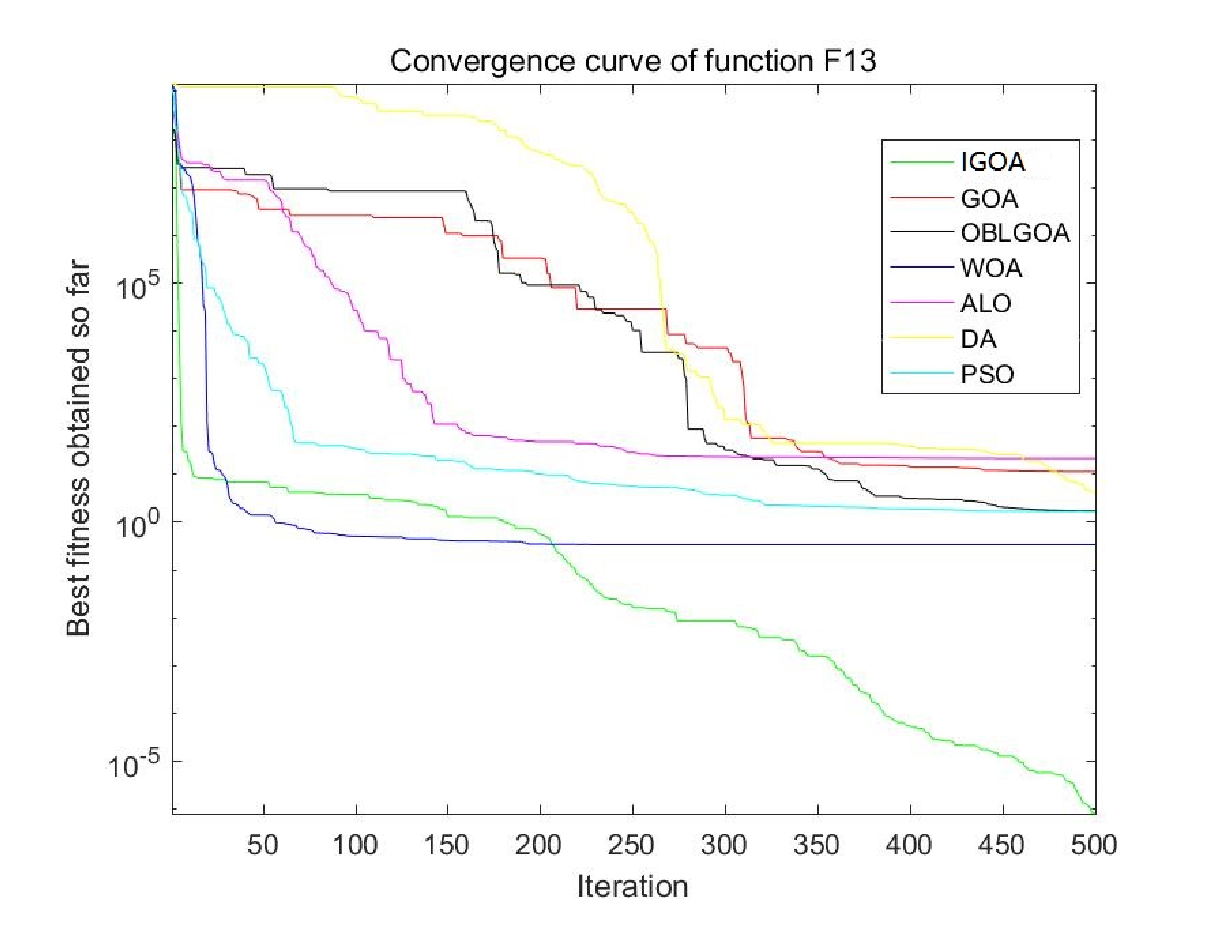
\includegraphics[width=.5\linewidth]{function_F13.eps}\hfill\\[0.5cm]

    \centering
    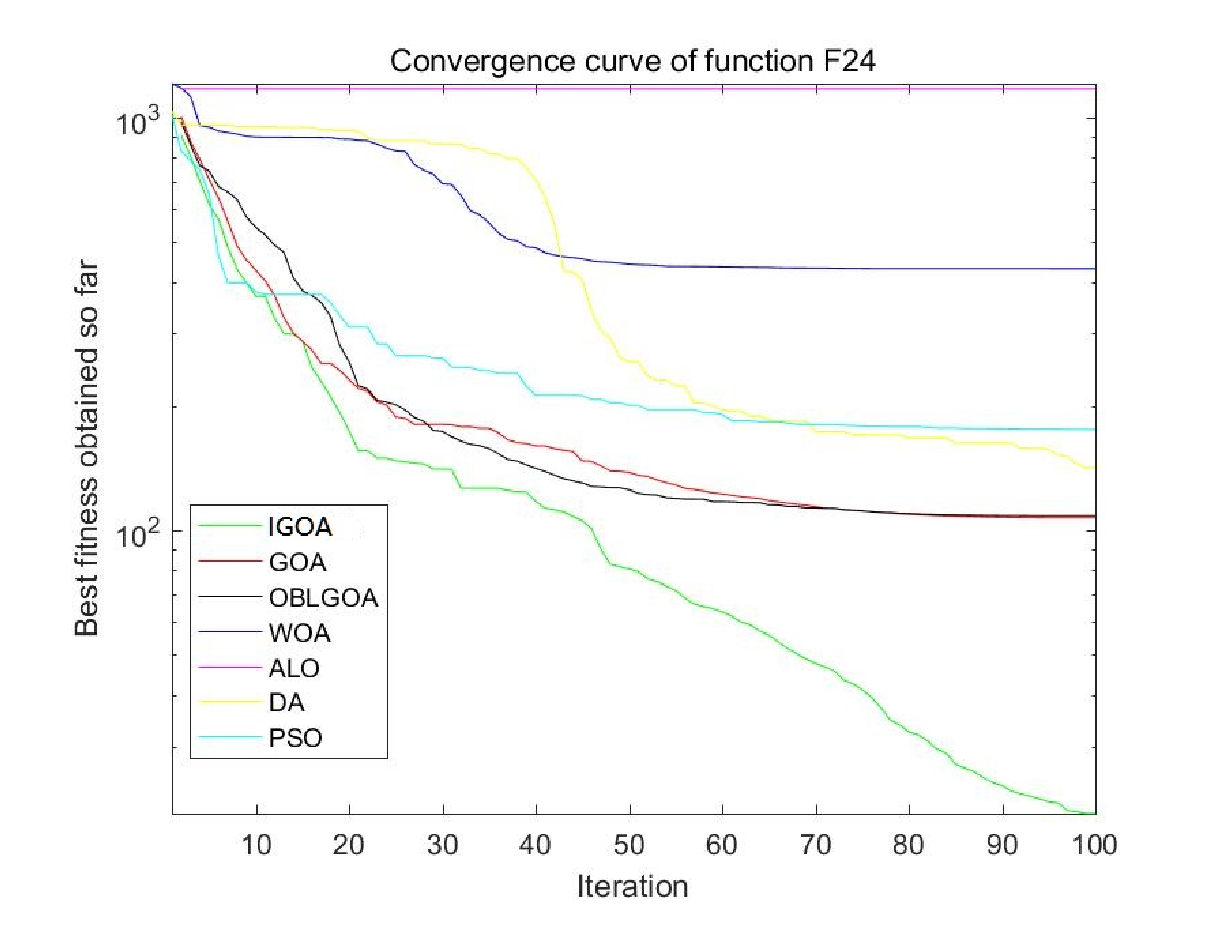
\includegraphics[width=.5\linewidth]{function_F24.eps}\hfill
    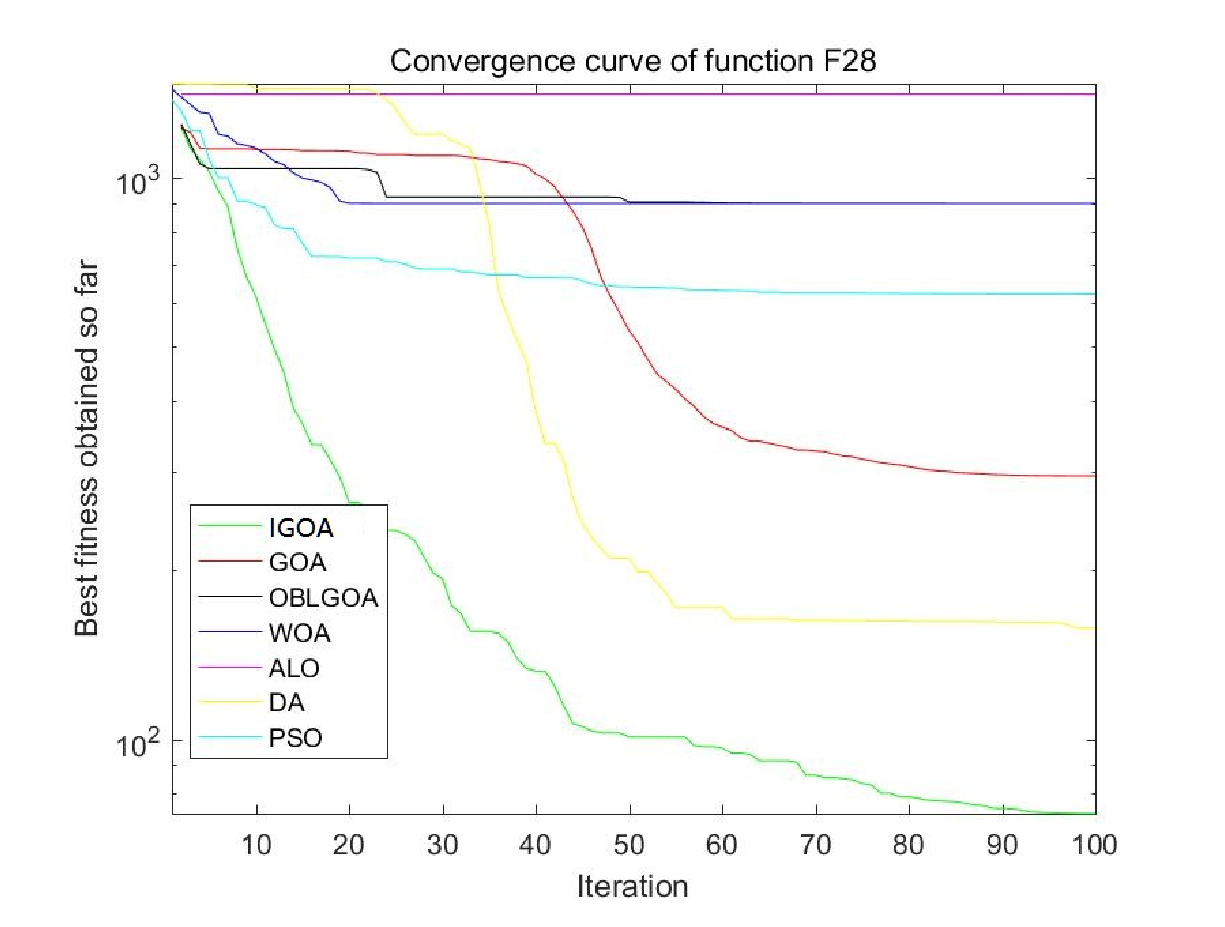
\includegraphics[width=.5\linewidth]{function_F28.eps}\hfill\\[0.5cm]

  \caption{7种算法在部分测试函数上搜索的收敛曲线图}
  \label{fig:IGOA_convergence_curve}
  \end{figure}


水平轴是当前迭代的次数,垂直轴是迄今为止所搜索到的最佳适应度值。为了使收敛曲线的表现力更明显,在垂直轴上使用对数。图\ref{fig:IGOA_convergence_curve}中的函数收敛曲线表明,相对于整个搜索过程,在大多数搜索过程中IGOA都可以保持较大的斜率。这种现象意味着所提出的非线性舒适区控制参数可以有助于充分利用每次迭代。曲线跨度在大多数函数中都是充分的,这也表明基于$L\acute{e}vy$飞行的局部搜索机制使算法更具创造性。在测试函数$F_3$、$F_4$、$F_7$和$F_{28}$中出现的突然下降,表明随机跳出策略可以帮助搜索跳出局部最优。算法在测试函数上的收敛曲线图表明,所提出的IGOA可以使搜索过程比其他搜索算法更快地收敛。

% The convergences rate of the algorithms are discussed in this part. The convergence curves of IGOA and all the other 6 algorithms for comparison over part of the benchmark functions are shown in \emph{Figure 2}. The horizontal axis is the number of the current iteration, and the vertical axis is the best fitness value obtained so far. To make the curve more distinguishable, the logarithm is used in the vertical axis. The curve image in \emph{Figure 2} indicates that IGOA can keep a large slope relatively for the entire search process in most of the search processes. This phenomenon can mean that the proposed nonlinear comfort zone parameter can contribute to making full utilization of every iteration. The curve span is ample in most of the functions, which can suggest that the local search mechanism based on $L\acute{e}vy$ flight makes the algorithm more creative. Some sudden drops of the curve occurred frequently in \emph{F3}, \emph{F4},\emph{F7}, and \emph{F28} show that the random jumping strategy can help the search jump out of the local optimum. The convergence curves demonstrate that the proposed IGOA can make the search process converge more rapidly than others generally.
\section{多终端协同服务的任务调度问题}\label{sec:task_scheduling_problems}
\subsection{问题描述}

任务调度问题是一种在云计算\cite{qiao2016efficient}、边缘计算\cite{guo2017energy}、海服务\cite{王劲林2015一种现场}等领域常见的问题。大量的用户会产生大量的任务。因此,当大量用户同时访问终端服务时,系统应该能够高效地处理这些任务,这是终端服务系统的一个重要问题,尤其是在终端资源有限的情况下。在任务调度问题中,一系列任务会到达任务调度中心,等待分配给特定的执行节点。
% Task scheduling problem is a common problem in cloud computing area\cite{qiao2016an}, edge computing area\cite{guo2017energy} and SEA Service System\cite{wang2015research}. Massive users produce massive tasks. Thus the system should handle the tasks efficiently when a large number of users ask the service at the same time, which can be an essential problem of the computing system, especially in resources constrained conditions. In task scheduling problems, a series of tasks arriving at the scheduling center wait to be allocated to a particular execution node. 

由于资源情况、工作负载、处理速度和任务类型的不同,执行节点在此问题中是异构的。不同的任务调度方案会产生不同的执行结果,一个优秀的任务调度解决方案可能会对整个系统服务效果产生很大影响。对于终端服务的提供商来说,将任务分配给合适的节点可以节省能源并且减少预算。而对于终端服务的使用者来所,将任务调度到高效节点可以减少等待时间并提高用户体验。
% The execution node might be heterogeneous in this problem because of the difference in the resource condition, workload, processing speed and the type of task. A different solution to task scheduling could lead to different consequence, and an excellent solution can affect a lot. For service providers, allocating a task to the proper node can save energy and reduce the budget. For service consumers, scheduling the task to the efficient node can decrease the waiting time and improve the user experience. 

% 任务调度问题是一个优化问题,也是一个NP难问题\cite{tawfeek2013cloud}。应用了许多算法来解决任务调度问题。一些基于最佳资源选择(BRS)的算法,如Max-Min,Min-Min和Sufferage,是解决任务调度问题的传统方法\ cite {qiao2016an}。当任务数量增加时,任务的维度也会增加,这会扩大搜索空间并使优化问题更加复杂。传统算法无法处理这种情况。近年来,许多元启发式算法被应用于解决任务调度问题。 Goldberg在1988年提出的遗传算法(GA)是一种着名的进化算法,它代表了一种解决任务调度问题的染色体调度方案。由于交叉和变异的操作,GA计算起来很复杂。粒子群算法(PSO)是Kennedy和Eberhard在1995年提出的经典元启发式算法.PSO将调度解决方案表示为离散粒子,并通过群体的个人最佳和全局最佳信息进行演化。 PSO很容易陷入局部最优,并且在处理多模态问题时表现不佳。
% Task scheduling problem can be an optimization problem, and it is an NP-hard problem\cite{tawfeek2013cloud}. Many algorithms are applied to solve the task scheduling problem. Some algorithms based on best resource selection(BRS) such as Max-Min, Min-Min, and Sufferage are traditional methods to solve task scheduling problems\cite{qiao2016an}. The dimension of the tasks can also increase when the number of tasks increases, which can enlarge the search space and make the optimization problem more complicated. The traditional algorithms could not handle this situation. In recent years many meta-heuristic algorithms were applied to solve the task scheduling problem. Genetic algorithm(GA) proposed by Goldberg in 1988 is a famous evolutionary algorithm, and it represents a scheduling scheme as a chromosome to solve the task scheduling problem. GA is complicated to calculate because of its operations of crossover and mutation. Particle Swarm Algorithm (PSO) is a classical meta-heuristic algorithm proposed by Kennedy and Eberhard in 1995. PSO represents a scheduling solution as a discrete particle and evolves by the information of the personal best and the global best of the swarm. PSO is easy to fall into local optimum, and it does not perform well when dealing with multimodal problems. 

本小节将所提出的IGOA算法应用于多终端协同服务的任务调度问题。将N个任务调度到M个节点的一种解决方案抽象表示为搜索空间中的一个位置,每一种解决方案都是一个N维离散向量。每个解决方案可以对应一个系统的完工时间和预算费用,并且可以通过完工时间和预算费用来计算适应度值。搜索单元集群通过IGOA算法的搜索策略在整个搜索空间中搜索最佳适应度值的位置,能够得到最优或近似最优的任务调度方案。
% Some recently proposed meta-heuristic algorithms are used such as DA, WOA, GOA and so on. In this work, the proposed IGOA is employed for task scheduling problems. A solution of N tasks scheduled to M nodes is abstracted as an N-dimension discrete vector which represents a position in the search space. Each solution can correspond to a makespan and a budget of the system, and a fitness value can be calculated with the makespan and budget. Several search agents search in the whole search space for the best fitness by the search strategy of IGOA.

\subsection{任务调度模型}
在本小节的研究中,假设用户启动\emph{N}个任务,这些任务分别为${T_1,T_2,...,T_N}$,终端服务系统有\emph{M}个节点可以用来处理任务,这些节点分别为$\{S_1,S_2,...,S_M\}$。任务调度模型描述如下。
% In this paper, we assume that users start \emph{N} tasks which are ${T_1,T_2,...T_N}$ and \emph{M} nodes which are $\{S_1,S_2,...S_M\}$ are waiting to handle them. The task scheduling model is described as follows.
\begin{enumerate}[]
    \item \emph{N}个任务的集合为$\{T_1,T_2,...T_N\}$,$T_i$代表第\emph{i}个任务所消耗的资源
    \item \emph{M}个节点的集合为$\{S_1,S_2,...S_M\}$,$S_j$代表第\emph{j}个节点所能提供的最大资源
    \item 只要某个节点能够提供某个任务执行所需要的足够资源,也就是$T_i \leq S_j$,该任务就可以在该节点上执行,
    \item 每个节点在同一时间只能执行一个任务,多个任务可以在同一个节点上排队执行
    \item 所有任务被分为\emph{K}种类型。表示任务类型的向量为$tot[N]$,$tot_i$代表第\emph{i}个任务的类型,取值为[1, K]中的整数
    \item 每个节点处理不同类型任务的能力不同。$mips[M,K]$是执行速度矩阵$mips_{j}^{k}$ 代表类型\emph{k}的任务在第\emph{j}个节点上执行时单位时间内消耗的资源数量。$et_{ij}$代表第\emph{i}个任务在第\emph{j}个节点上执行所消耗的时间,计算方式如公式\ref{equ:task_scheduling_etij}所示。
    \begin{eqnarray}\label{equ:task_scheduling_etij}
        et_{ij}= \begin{cases}
            \frac{T_i}{mips_{j}^{tot_i}} & task\  i\  runs\  on\  node\  j \\
            0&task\  i\  does\  not\  runs\  on\  node\  j 
            \end{cases} 
    \end{eqnarray}
    \item 第\emph{j}个节点的执行时间$st_j$是通过将在第\emph{j}个节点上执行的所有任务的执行时间相加得到的。计算方法如公式\ref{equ:task_scheduling_stj}所示。
    \begin{eqnarray}\label{equ:task_scheduling_stj}
        st_{j}=\sum_{i=1}^{N} et_{ij}
    \end{eqnarray}
    总的执行时间\emph{Makespan}所有节点的执行时间取最长值。计算方法如公式\ref{equ:task_scheduling_makespan}所示。
    \begin{eqnarray}\label{equ:task_scheduling_makespan}
        Makespan=\max\{st_j | j=1,2,3...M\}
    \end{eqnarray}
    \item 工作节点在执行任务的时候会产生额外的费用开销。费用只与工作节点的工作时间有关,不论工作节点上执行的是什么类型的任务。节点的费用向量为$bps[M]$,代表着第\emph{j}个节点在单位时间内产生的额外费用开销。
    \item  总的费用\emph{Budget}是通过将所有节点产生的费用相加得到的。\emph{Budget}的计算方法如公式\ref{equ:task_scheduling_makespan}所示。
    \begin{eqnarray}\label{equ:task_scheduling_budget}
        Budget=\sum_{j=1}^{M} (st_j \times bps_j)
    \end{eqnarray}
    \item 时间和费用是从两个方面来描述任务调度问题的开销情况的,因此需要一个统一的评估适应度。在这里,任务调度问题的评估适应度被定义为时间和费用通过权重参数$\alpha$和$\beta$进行结合的结果。评估适应度\emph{fitness}的计算如公式\ref{equ:task_scheduling_fitness}所示。
    \begin{eqnarray}\label{equ:task_scheduling_fitness}
        fitness=\alpha Makespan + \beta Budget
    \end{eqnarray}
    \item 搜索过程是连续的,但问题的解决方案是离散的。所以当每个循环迭代的过程结束后,所有的搜索单元都应该向距离其最近的整数位置进行调整。
    \item 同一个节点上执行的两个任务之间的切换时间被忽略。边缘节点之间的传输时间也被忽略不计。
\end{enumerate}
\subsection{实验结果}
在此任务调度模块中,\emph{N}个任务被分为\emph{K}种类型,\emph{M}个工作节点正在准备处理它们。任务调度模块的参数选择的细节取决于具体问题,这里不再进行讨论。在本小节的工作中,不失一般性地,\emph{K},\emph{N}和\emph{M}分别设置为4,10和5。 为了平衡\emph{Makespan}和\emph{Budget}对\emph{fitness}的影响,系数$\alpha$和$\beta$设置为0.7和0.3。上述参数设定如公式\ref{eqn:task_scheduling_KNM}所示。
% In this task scheduling module, \emph{N} tasks are divided into \emph{K} types, and \emph{M} working nodes are preparing to handle them. The specifics of the parameter selection of the task scheduling module depend on the specific problem and will not be discussed here. In this work, without loss of generality, \emph{K}, \emph{N} and \emph{M} are set to 4,10 and 5 respectively. To balance the impact of \emph{Makespan} and \emph{Budget} on \emph{fitness}, the coefficients $\alpha$ and $\beta$ are set to 0.7 and 0.3. Those parameters mentioned above are set as follows.
\begin{eqnarray}\label{eqn:task_scheduling_KNM}
    K=4;\ N=10;\ M=5;\ \alpha=0.7;\ \beta=0.3; 
\end{eqnarray}

向量\emph{T}, \emph{tot}, \emph{S}, \emph{bps}以及矩阵\emph{mips}的设置如表\ref{tab:resource_type_tasks}所示。
% The vector T, tot, S and bps, and the matrix mips are set as \emph{Table 10-12}.
\begin{table}[!htbp]
    \centering
    \caption{任务类型及任务消耗资源情况}\label{tab:resource_type_tasks}
    \renewcommand\arraystretch{1.3} 
    % \scriptsize
\begin{tabular}{*{11}{c}}
    \hline
   task& 1& 2& 3& 4& 5& 6& 7& 8& 9& 10\\
    \hline
   T & 40& 20& 30& 40& 25& 35& 45& 10& 5& 10 \\
    \hline
   tot &1& 1& 1& 2& 2& 2& 3& 3& 4& 4 \\
    \hline
   
   \end{tabular}
\end{table}

\begin{table}[!htbp]
    \centering
    \caption{节点拥有资源及bps}\label{tab:resource_bps_nodes_tasks}
    \renewcommand\arraystretch{1.3} 
    % \scriptsize
\begin{tabular}{*{6}{c}}
    \hline
   node& 1& 2& 3& 4& 5\\
    \hline
   S & 100& 50& 150& 100& 80 \\
    \hline
   bps &0.5& 0.2& 0.8& 0.1& 0.5 \\
    \hline
   
   \end{tabular}
\end{table}

\begin{table}[!htbp]
    \centering
    \caption{任务和节点的mips}\label{tab:mips_tasks_nodes}
    \renewcommand\arraystretch{1.3} 
    \begin{tabular}{|c|c|c|c|c|c|}
        \hline
        
        {{$mips_j^k$} }& \multicolumn{4}{|c|}{k:1-4} \\
        
        \hline
        \multirow{5}*{j:1-5}&5& 2& 10& 8\\
        \cline{2-5}
        &2& 4& 2& 1\\
        \cline{2-5}
        &8& 10& 10& 5\\
        \cline{2-5}
        &2& 1& 3& 4\\
        \cline{2-5}
        &5& 5& 8& 8\\
        \hline
        \end{tabular}
\end{table}   

在本小节的工作中,所提出的IGOA与另外6个算法进行了比较,包括GOA、WOA、ALO、DA、PSO和OBLGOA。每种算法使用30个搜索单元进行搜索。为了减少意外因素的影响,对每种算法进行了30次独立测试,计算并比较了测试结果的平均值,标准差,最优值和最差值等统计数据。实验结果如表\ref{tab:results_task_scheduling}所示。
% In this work, 6 algorithms were compared with the proposed IGOA. 30 search agents were employed in each algorithm. In order to reduce the impact of accidental factors, every algorithm was tested for 30 times and the statistical data such as average value, standard deviation, best value and worst value were calculated and compared. The result of the experiment is listed as \emph{Table 13}. 
\begin{table}[!htbp]
    \centering
    \caption{任务调度实验结果}\label{tab:results_task_scheduling}
    \renewcommand\arraystretch{1.3} 
    % \scriptsize
\begin{tabular}{*{6}{c}}
    \hline
    algorithm&average&std&best&worst&promotion\\
    \hline
    IGOA& 13.50&	0.62&	12.63&	14.62&	0    \\
    \hline
    GOA & 14.95&	0.82&	13.50&	16.67&	9.7\%    \\
    \hline
    WOA &14.08&	0.75&	13.02&	15.93&	4.1\%    \\
    \hline
    ALO &19.83&	2.89&	16.02&	26.76&	31.9\%    \\
    \hline
    DA &19.00&	2.49&	15.62&	26.81&	29.0\%    \\
    \hline
    PSO &17.93&	1.68&	13.96&	22.29&	24.7\%\\
    \hline
    OBLGOA &14.85&	0.74&	13.30&	16.27&	9.1\%\\
    \hline
   
   \end{tabular}
\end{table}

从表\ref{tab:results_task_scheduling}中可以看出,实验结果表明,所提出的IGOA在所有领域都优于其他算法。IGOA在平均值方面可以做得最好。IGOA拥有最小的标准差,说明该算法相比其他算法更加稳定。IGOA可以找到所有算法中的最优解,并且能够控制找到最差解的值。与其他6种算法相比,IGOA可以将平均值分别提升9.7\%,4.1\%,31.9\%,29.0\%,24.7\%和9.1\%。
% The result of the experiment demonstrated that the proposed IGOA outperformed the other algorithms in all field. IGOA can do best in average values, and it can be more stable for the smallest standard deviation. It can have the ability to find the best solution over all the algorithms, and it can control the worst value which it can find. Compared with the other algorithms, IGOA can promote the average values respectively by 9.7\%, 4.1\%, 31.9\%, 29.0\%, 24.7\%, and 9.1\%.

\section{本章小结}\label{sec:task_scheduling_summary}

为了在终端资源有限且终端资源异构性强的情况下,合理调度任务请求到更合适的执行节点上,使得任务总体开销更小,减少响应时间,提高用户体验,本章基于一种群体智能的演进式优化算法————蝗虫优化算法,提出一种带有随机跳出机制的动态权重蝗虫优化算法来解决优化问题。该算法在原有蝗虫优化算法的基础上,增加了基于完全随机跳出因素的跳出机制,来提高算法的跳出局部最优的能力。另外,还根据搜索阶段的不同,使用动态的权重参数来代替原算法中的线性递减搜索单元权重参数,帮助算法在不同的搜索阶段获得更大的迭代收益。经过一系列测试函数的实验验证,所提出的带有随机跳出机制的动态权重蝗虫优化算法能够有效提高优化算法的搜索精度及收敛速度。在此基础上进一步提出一种改进蝗虫优化算法,并将其应用于解决多终端任务调度问题。该算法引入变形的sigmoid函数作为非线性舒适区调节参数,增强算法的搜索能力。同时,提出基于$L\acute{e}vy$飞行的局部搜索机制,让搜索单元在局部拥有一定的“搜索视觉”,提高算法的局部搜索能力。另外,该算法还使用基于线性递减参数的随机跳出策略,增强算法跳出局部最优能力,并将成功跳出的结果影响力维持若干次迭代。经过一系列测试函数和标准测试集的实验,实验结果表明所提出的改进蝗虫优化算法能够有效提高优化算法的搜索精度、稳定性、搜索到更优解的可能性及收敛速度。最后提出了多终端协同服务任务调度问题的数学模型,并将提出的改进蝗虫优化算法应用到该问题的求解过程中。实验结果证明,所提出的改进蝗虫算法在求解终端上任务调度问题时能够得到很好的效果。

本章所涉及的研究成果包括:

论文2篇:“A Dynamic Weight Grasshopper Optimization Algorithm with Random Jumping”(3rd International Conference on Computer, Communication and Computational Sciences (IC4S2018),EI会议,已录用)。

“An Improved Grasshopper Optimization Algorithm for Task Scheduling Problems”(International Journal of Innovative Computing, Information and Control (IJICIC),EI期刊,已录用)。
